\documentclass[a4paper,article,14pt]{extarticle}

% Подключаем главный пакет со всем необходимым
\usepackage{spbudiploma_tempora}

% Пакеты по желанию (самые распространенные)
% Хитрые мат. символы
\usepackage{euscript}
% Таблицы
\usepackage{longtable}
\usepackage{makecell}
\usepackage{tabularx}
% Картинки (можно встявлять даже pdf)
\usepackage[pdftex]{graphicx}

\usepackage{amsthm,amssymb, amsmath}
\usepackage{textcomp}
\DeclareMathOperator{\sech}{sech}
\usepackage{gensymb}
\usepackage{natbib}

%\setcitestyle{authoryear,open={((},close={))}} %Citation-related commands

\begin{document}

% Титульник в файле titlepage.tex
% --------------------- Титульник ВКР СПбГУ -----------------------------
% Автор: Тоскин Николай, itonik@me.com
% Если заметили ошибку, напишите на email
% Если хотите добавить изменение самостоятельно:
% https://github.com/itonik/spbu_diploma/
% Использованы материалы:
% habr.com/ru/post/144648/
% cpsconf.ru
% Документы ниже могут уже быть неактуальны, тем не менее за годы ничего
% нового не появилось
% Текст:
% http://edu.spbu.ru/images/data/normativ_acts/local/20181030_10432_1.pdf
% Титульный лист:
% http://edu.spbu.ru/images/data/normativ_acts/local/20180703_6616_1.pdf
% -----------------------------------------------------------------------

% Титульный лист диплома СПбГУ
% Временное удаление foot на titlepage
\newgeometry{left=30mm, top=20mm, right=15mm, bottom=20mm, nohead, nofoot}
\begin{titlepage}
\begin{center}
\vspace*{95mm}

% \textbf{Санкт--Петербургский}
% \textbf{государственный университет}

% \vspace{35mm}

% \textbf{\textit{\large Скрябина Мария Николаевна}} \\[8mm]
% % Название
% \textbf{\large Выпускная квалификационная работа }\\[3mm]
\textbf{\textit{\large Видимые с ребра галактики в глубокой полосе SDSS Stripe82}}

% \vspace{20mm}
% Уровень образования: специалитет\\
% Специальность: 03.05.01 «Астрономия»\\
% Специалитет СМ.5012.2016 «Астрономия» \\
% Профиль: «Наблюдательная астрофизика»\\[25mm]


% Научный руководитель, рецензент
% \begin{flushright}
% \begin{minipage}[t]{0.5\textwidth}
% {Научный руководитель:}
% \smallskip\\

% к.ф.-м.н., ведущий научный сотрудник\\ Савченко С.С. \\ 
% Кафедра астрофизики\\

% {Рецензент:} \\
% к.ф.-м.н., старший научный сотрудник Мосенков А. В.\\
% ГАО РАН
% \vspace{10mm}


% \end{minipage}
% \end{flushright}

\vfill 

% {Санкт-Петербург}
\par{\the\year{} г.}
\end{center}
\end{titlepage}
% Возвращаем настройки geometry обратно (то, что объявлено в преамбуле)
\restoregeometry
% Добавляем 1 к счетчику страниц ПОСЛЕ titlepage, чтобы исключить 
% влияние titlepage environment
\addtocounter{page}{1}

% --------------------- Титульник ВКР СПбГУ -----------------------------
% Автор: Тоскин Николай, itonik@me.com
% Если заметили ошибку, напишите на email
% Если хотите добавить изменение самостоятельно:
% https://github.com/itonik/spbu_diploma/
% Использованы материалы:
% habr.com/ru/post/144648/
% cpsconf.ru
% Документы ниже могут уже быть неактуальны, тем не менее за годы ничего
% нового не появилось
% Текст:
% http://edu.spbu.ru/images/data/normativ_acts/local/20181030_10432_1.pdf
% Титульный лист:
% http://edu.spbu.ru/images/data/normativ_acts/local/20180703_6616_1.pdf
% -----------------------------------------------------------------------

% Титульный лист диплома СПбГУ
% Временное удаление foot на titlepage
\newgeometry{left=30mm, top=20mm, right=15mm, bottom=20mm, nohead, nofoot}
\begin{titlepage}
\begin{center}

% \textbf{SAINT--PETERSBURG}
% \textbf{STATE UNIVERSITY}

% \vspace{35mm}

% \textbf{\textit{\large Skriabina Mariia}} \\[8mm]
% % Название
% \textbf{\large Graduation Thesis}\\[3mm]
\vspace*{95mm}
\textbf{\textit{\large Edge-on galaxies in the deep SDSS Stripe82}}

% \vspace{20mm}
% The educational level: Specialty\\
% The educational program: 03.05.01 «Astronomy»\\
% Specialization: «Observational astrophysics»\\[25mm]


% % Научный руководитель, рецензент
% \begin{flushright}
% \begin{minipage}[t]{0.5\textwidth}
% {Scientific supervisor:} \\
% Savchenko Sergey \\ 

% {Reviewer:} \\
% Mosenkov Alexandr\\

% \vspace{10mm}


% \end{minipage}
% \end{flushright}

\vfill 

% {Saint-Petersburg}
\par{\the\year{}}
\end{center}
\end{titlepage}
% Возвращаем настройки geometry обратно (то, что объявлено в преамбуле)
\restoregeometry
% Добавляем 1 к счетчику страниц ПОСЛЕ titlepage, чтобы исключить 
% влияние titlepage environment
\addtocounter{page}{1}


% Содержание
\tableofcontents
\pagebreak
% Разделы
\specialsection{Введение}
За последние десятилетия огромную роль в изучении Вселенной стали играть исследования, основанные на глубоких и очень глубоких изображениях космических объектов. Связано это с техническим прогрессом и появлением телескопов, способных различить структуры, поверхностная яркость которых достигает 30 mag/arcsec$^2$. Возникновение такого большого количества наблюдательных данных создает огромный простор для новых исследований объектов, которые ранее были нам недоступны для наблюдений. 

В частности, одна наиболее интересная для изучения область неба, это полоса Sloan Digital Sky Survey (SDSS) Stripe 82 – полоса шириной 2.5 градуса вдоль небесного экватора с координатами -50\degree < R.A. < 60\degree, -1.25\degree< Dec < 1.25\degree и  с общей площадью 275 квадратных градусов во всех пяти фильтрах SDSS. Преимущества данной полосы заключаются в ее расположении: в первую очередь,  полоса Stripe 82 доступна для большинства наземных телескопов, что позволяет производить вспомогательные спектроскопические и фотометрические наблюдения. Во-вторых, эта полоса охватывает области от очень низкого, до высокого галактического поглощения, что может быть полезно для анализа рассеяния излучения пыли нашей Галактики. Конкретно для нашего исследования полоса Stripe 82 имеет преимущества в том, что в течение нескольких десятков лет в данной области были получены изображения неба порядка 80 раз во всех пяти SDSS фильтрах ugriz, в результате чего, мы имеет дело с кадрами, глубина которых отличается на 2 mag/arcsec$^2$ и более (для сравнения стандартные кадры SDSS достигают глубины 26.5 mag/arcsec$^2$ в фильтре r, тогда как средний предел по глубине изображений, загруженных из базы данных Stripe 82 в том же диапазоне, составляет 28.6 mag/arcsec$^2$). \footnote{\url{http://research.iac.es/proyecto/stripe82/}}

Глубина изображений в SDSS полосе Stripe 82 позволяет нам исследовать структуры низкой поверхностной галактик. Имея две выборки галактик с наблюдаемыми и отсутствующими приливными структурами мы можем сравнить средние толщины звездных дисков для обеих выборок (например, в работе \cite{1997A&A...324...80R} отношение радиального и вертикального масштабов $h_r/z_0$ примерно в 1.5-2 раза больше для галактик с приливными структурами, что можно объяснить большими дисперсиями скоростей звезд в вертикальном направлении у галактик, подверженных слиянию с другими объектами). Данная зависимость еще не является хорошо исследованной, поэтому в нашей работы мы попробуем пролить чуть больше света на вышеописанный вопрос.

Проектов, в рамках которых были обработаны изображения SDSS полосы Stripe 82 достаточно много. Один из них -- IAC Stripe 82 Legacy Project \footnote{\url{http://research.iac.es/proyecto/stripe82/}}. Основная цель проекта IAC Stripe 82 Legacy заключается в сохранении структур низкой поверхностной яркости во всех пространственных масштабах и масштабах интенсивности, используя неагрессивный метод вычитания фона неба. В нашей работе мы использем данные из IAC Stripe 82 Legacy Project, чтобы создать каталог галактик с ребра (далее ES82 – Edge-on galaxies in sdss Stripe 82) в полосе Stripe 82, с возможностью последующего исследования глубоких изображений этих объектов, выявления структур низкой поверхностной яркости (LSB – Low Surface Brightness), таких как полярные кольца, арки, хвосты и т.д., свидетельствующие о возможном взаимодействии галактик с их окружением, анализа параметров вертикальной и радиальной структуры звездных дисков спиральных галактик на основе данных о поверхностной фотометрии галактик, что может дать ответы на многие вопросы, связанные с образованием и эволюцией этих объектов. 





\section{Основные этапы работы}
В процессе работы были выделены следующие этапы ее выполнения:
\begin{enumerate}
    \item Отбор потенциальных галактик видимых с ребра, используя каталог объектов, полученный при помощи SExtractor  в работе Fliri J., Trujillo I \cite{2016MNRAS.456.1359F}. в рамках проекта IAC Stripe 82 Legacy Project, а также каталогов EGIS \cite{2017MNRAS.465.3784B} и Galaxy Zoo \cite{2017yCat..74613663H} (критерии отбора: угловой размер галактики, диаметр 25 изофоты,  не менее 30 arcsec, сжатие галактики $\frac{b}{a}$ менее 0.3).
    \item Проведение визуального отбора и усовершенствование выборки.
    \item Обработка изображений галактик в фильтрах g, r, i, rdeep (разворот, обрезка).
    \item Создание цветных RGB изображений.
    \item  Совершенствование выборки на основании полученных RGB изображений.
    \item Переопределение размеров галактик для более точной обрезки изображений (выполнено при помощи SAOImageDS9).
    \item Создание масок (для изображений в фильтрах rdeep, r)\footnote{Изображения-маски имеют размер как у изображения с исследуемой галактикой, но на нем помечены лишние объекты, которые попали на изображение. В процессе создания суммарных изображений или фотометрической декомпозиции не должны участвовать пиксели, которые заведомо
фоном неба не являются, их следует замаскировать.}, которые будут использоваться для создания суммарных изображений и фотометрической декомпозиции. 
    \item Создание суммарных изображений.
    \item Отбор галактик, обладающих структурами низкой поверхностной яркости (хвосты, арки, мосты, полярные кольца, диффузные оболочки и др.) на основании контрастных, цветных RGB изображений, изображений из обзора Legacy\cite{2019AJ....157..168D}, HSC-SSP (Hyper Suprime-Cam Subaru Strategic Program)\cite{2022PASJ...74..247A}.
    \item Классификация объектов по различным структурам низкой поверхностной яркости.
    \item Приведение статистики проклассифицированных структур.
    \item Выполнение одномерной фотометрической декомпозиции с целью определения нулевого приближения модельных параметров галактик и использования их в последующем этапе -- двумерной фотометричксой декомпозиции.
    \item Выполнение двумерной фотометрической декомпозиции.
    \item Анализ ее результатов.
    % \item Выполнение двумерной фотометрической декомпозиции для изображений галактик с замаскированной пылевой полосой.
    % \item Анализ полученных на предыдущих этапах параметров (соотношение вертикального и радиального масштабов,  распределение галактик выборки, по звездным величинам, по красным смещениям, сравнение толщин звездных дисков для галактик с наблюдаемыми и ненаблюдаемыми приливными структурами и др.).

\end{enumerate}
\section{Выборка}
После первичного отбора галактик с ребра выборка включала 1167 объектов из каталога Fliri J., Trujillo I. \cite{2016MNRAS.456.1359F}, полученного в рамках проекта IAC Stripe 82 Legacy Project при помощи Sourse Extractor (сокращенно: Sextractor), а также каталогов EGIS\cite{2014ApJ...787...24B} и Galaxy Zoo \cite{2017yCat..74613663H}.
Работа программы SExtractor сводится к тому, что на подаваемом на вход
изображении в фитс-формате (fits) находятся объекты и вычисляются
некоторые их параметры, такие как размер, видимая звездная величина, эллиптичность, позиционный угол и пр. 
Для отбора объектов в каталог использовались следующие параметры SExtractor: $A\_IMAGE$, $B\_IMAGE$ -- большая и малая полуоси галактики, $KRON\_RADIUS$ -- радиус Крона. 
Критерии для отбора галактик в каталок:
\begin{itemize}
    \item Угловой размер галактики (радиус 25 изофоты $r_{25}$ -- радиус изофоты на котором угловая поверхностная яркость галактики достигает  $25 mag/arcsec^2$) не менее 15 arcsec. Данный параметр нам изначально не известен, но с помощью базы данных LEDA\footnote{\url{http://leda.univ-lyon1.fr/}} мы можем узнать размер $r_{25}$  для некоторых галактик из выборки и найти коэффициенты взаимосвязи радиуса Крона $KRON\_RADIUS$, известного параметра и $r_{25}$, тем самым усовершенствовав выборку объектов.
    \item Сжатие галактики ($B\_IMAGE/A\_IMAGE$) менеее 0.3
\end{itemize}

После были скачаны jpg изображения для полученного списка галактик и проведен визуальный отбор, в результате которого были удалены из выборки галактики, явно не относящиеся к галактикам, видимым с ребра: галактики, находящиеся под углом наклона менее 80-85 градусов (те, у которых видна плоскость диска, возможные спирали. В случае галактики, видимой точно с ребра, ветви не должны быть видны, в то время как даже при небольшом наклоне они могут стать видимыми), другие объекты.
Также проведенный визуальный анализ цветных RGB изображений позволил сузить список изучаемых объектов до 831 (важно отметить, что в данной выборке не все галактики являются галактиками с ребра, часть  объектов, не смотря на угол наклона < 85º, оставлены по причине наличия интересных структурных особенностей). Каталог, который включает только галактики с ребра состоит из 710 объектов.

В процессе работы были вручную переопределены размеры и позиционные углы у $40\%$ галактик, так как их изначальные значения были далеки от реальности.
Визуальный анализ цветных и контрастных изображений позволил сделать выводы о небольшом количестве галактик в полосе Stripe 82, обладающих структурами низкой поверхностной яркости (подробнее в разделе "Статистика проклассифицированных структур").  
\section{Полнота выборки}
С целью оценить полноту каталога нами был выполнен $V/V_m$ тест, описанный в работе \citep{1979ApJ...231..680T}. Мы расчитали для каждой галактики объем сферы \textit{V} с радиусом, равным расстоянию до объекта D, выражающимся следующим образом: $D = d/\theta$, где d -- линейный диаметр галактики, $\theta$ -- угловой. Также был посчитан объем сферы $V_m$, радиус которой, это максимальное расстояние $D_m$, на котором должна находиться галактика и всё еще принадлежать нашей выборке объектов. С учетом того, что $D_m = d/\theta_L$, данное расстояние будет соответствовать объекту выборки с наименьшим угловым размером, в нашем случае $\theta_L$ = 6.38 arcsec (за значение углового размера мы берем значение большой полуоси галактики \textit{SMA}). 
Отношение объемов $V/V_m =  (\theta_L/\theta)^3$. Среднее значение отношения этих объемов, которое мы будем обозначать как $\langle V/V_m \rangle$ должно равняться 0.5 для объектов равномерно распределенных в Евклидовом прострастве в случае, если выборка полная. 

Вычисляя это значение для каталога объектов, последовательно исключая объекты с маленькими угловыми размерами мы приходим к тому, что для $SMA>18$ arcsec (55$\%$ выборки) наша выборка, по существу, полна: в фильтре \textit{r} $\langle V/V_m \rangle = 0.489$.

\section{Данные и их обработка}
Работа производилась со "sky rectified"$\textrm{ }$ изображениями (с уже вычтенным фоном неба), полученными в рамках IAC Stripe 82 Legacy Project.  Используемые фильтры: gri (этап с созданием цветных RGB изображений, фотометрическая декомпозиция), rdeep (этапы с созданием масок, суммарных изображений). 
В процессе выполнения работы были написаны python-скрипты для маскирования, отбора, классификации галактик, скачивания данных, склейки полей.
Для обработки изображений (центрирование на объект, разворот галактики, обрезка изображения, создание rgb изображений, создание суммарных изображений) был использован полуавтоматический пакет для обработки и анализа изображений IMage ANalysis (IMAN)\footnote{\url{https://bitbucket.org/mosenkov/iman_new/src/master/}} и дополнительные python-скрипты. 

С учетом того, что использовались sky rectified изображения, вычет фона неба не производился. Порядок действий по обработке изображений, проводимый в процессе данной работы выглядит следующим образом:
\begin{enumerate}
    \item \textit{Загрузка данных}. Из IAC Stripe 82 Legacy Project были загружены поля в фильтрах r,g,b,rdeep, файлы с psf изображением \footnote{psf (point spread function) -- изображения, описывающие картину, получаемую системой формирования изображения при наблюдении точечного источника или точечного объекта.}, weight-изображения \footnote{weight - изображения, это така называемые карты весов. Имеют тот же размер, что и соответствующее ему изображение с исследуемой галактикой. Только если в обычном fits-изображении с галактикой каждому пикселю соответсвует его значение интенсивности, то в случае weight-файла, каждому пикселю соответсвует его "вес". Этот "вес" вычисляется как $w_i = 1/\sigma_i^2.$
i }
    \item \textit{Первичная обрезка изображения} в фильтрах g,r,i,rdeep с центрирование на объект. Зная координаты центра галактики мы можем вырезать из скачанного поля квадрат, достаточно большой, чтобы не потерять в процессе дальнешей обработки структуры низкой поверхностной яркости и части галактики (квадрат со стороной $\approx$ 10 размеров большой полуоси галактики). Данный этап позволяет быстрее выполнить последующие этапы обработки, например, разворот изображение вокруг центра галактики.
    \item \textit{Разворот галактики}, чтобы та располагалась горизонтально на изображении. На данном этапе используем известные нам значения позиционных углов. В процессе выполнения работы было обнаружено, что примерно для 40 $\%$ выборки изначальные значения PA, определеные при промощи SExtractor, являются неточными. Поэтому для данной категории объектов углы были переопределены методом вписывания эллипса, описывающего внешние изофоты галактики, в программе SAOImage DS9 \cite{2003ASPC..295..489J}. Новые значения позиционных углов были внесены в таблицу и использованы при повторном развороте изображений и анализе параметров объектов выборки.
    \item \textit{Конечная обрезка изображений}. Размер полученного поля составляет 6 размеров больших полуосей галактик. 
    \item \textit{Загрузка соседних полей} в случае, когда галактика находится на границе полей. Склейка осуществлялась при помощи программы SWarp. После осуществлялся повтор предыдущих шагов (обрезка, разворот). Все этапы с центрированием, обрезкой и разворотом производились также с weight-файлами, чтобы в результате каждому пикселю на изображении с галактикой соответствовал его вес в weight-файле.
    \item \textit{Создание масок}. Для данного этапа была создана программа, написанная на языке программирования python. Основной пакет, используемый в скрипте, это пакет \textit{photutils}. Он позволяет выделить на изображении некоторые сегменты, отличающиеся друг от друга по яркости. Каждому сегменту на сегментационной карте соответсвует определенный индекс. В случае, когда сторонний источник находится очень близко к галактике или даже проецируется на нее (то есть перекрывает ее тело), мы можем использовать "деблендинг", то есть разделение сегментов на еще меньшие сегменты, чтобы выделить из них относящиеся к галактике, и не относящиеся к ней. Удаляя из сегментационной карты все сегменты, относящиеся к исследуемому объекту, и оставляя сегменты, покрывающие сторонние источники, мы ликвидируем вклад излучения других объектов из анализа. Пример сегментационной карты, изображения, с наложенной маской приведен на рисунке \ref{fig:mask}.
    \item Создание суммарных\footnote{Суммарное изображение представляет собой сумму изображений в фильтрах r,g,b. Оно является более глубоким и контрасным, позволяющим более чётко видеть структуры низкой поверхностной яркости.} изображений, цветных RGB \footnote{Принцип создания RGB изображения основывается на принципе, в соответствии с которым каждому значению цвета пикселя (например, g-r или r-i) соответствует уникальный цвет на RGB изображении.} изображений.
    \item \textit{Обрезка и разворот}, выполненные для последующей фотометрической декомпозиции. На этом этапе важно, чтобы тело галактики занимало большую часть изображения, что ускоряет сам процесс декомпозиции и минимизирует возможность соседних объектов влиять на результат. Поэтому итоговый размер прямоугольного изображения составляет 3 соответсвующих полуосей галактики для каждой из сторон.
\end{enumerate}

\begin{figure}[ht]

    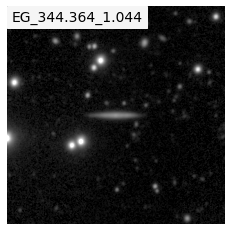
\includegraphics[width=.33\textwidth]{images/data_no_mask.png}\hfill
    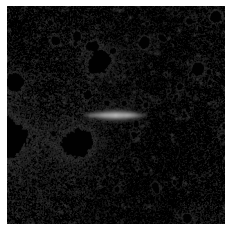
\includegraphics[width=.33\textwidth]{images/data_with_mask.png}\hfill
    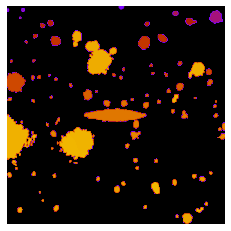
\includegraphics[width=.33\textwidth]{images/segm.png}\hfill

    \caption{Левая панель -- пример изображения галактики из выборки, центральная панель -- изображение той же галактики с наложенной маской, правая панель -- сегментационная карта для этой же галактики. }\label{fig:mask}
\end{figure}

\section{Классификация структур низкой поверхностной яркости}
В процессе визуального анализа суммарных и цветных RGB изображений было отобрано 43 галактики, имеющие приливные структуры низкой поверхностной яркости. Для более точного определения структур также использовались изображения из обзоров DESI Legacy Imaging Survey\cite{2019AJ....157..168D}, Hyper Suprime-Cam Subaru Strategic Program\cite{2022PASJ...74..247A}. 
Наблюдаемые структуры:
\begin{enumerate}
    \item Приливные хвосты -- протяженные структуры, состоящие из звезд и газа, часто образующиеся в результате крупных слияний галактик. (Рис. \ref{fig:tails})
    \item Диффузные оболочки. Под ними подразумеваем слабые протяженные гало вокруг дисков галактик, состоящие из старых звезд. Оболочки также могут являться признаком малых слияний в прошлом.(Рис. \ref{fig:shells})
    \item Мосты -- еще один подвид протяженных вытянутых структур, состоящих из звезд и газа, по сути, представляющие собой перетекание вещества от одного объекта к другому. (Рис. \ref{fig:bridges})
    \item Арки -- структуры вокруг галактики, имеющие аркообразную форму.(Рис.  \ref{fig:arcs})
    \item Остатки спутников, деформированные в процессе малого слияния. (Рис. \ref{fig:debris})
\end{enumerate}
Приливные структуры не ограничиваются списком перечисленных выше. Данные LSB структуры являются наиболее часто встречающимися в рамках нашего исследования (подробнее ознакомиться с темой галактик с приливными структурами можно, например в работе \citep{2019MNRAS.483.1470R}). Параметры галактик, обладающих приливными структурами, приведены в таблице \ref{tab:tab1}.
\begin{longtable}{|l|l|l|l|l|l|l|}
\caption{Параметры галактик из каталога ES82 обладающих приливными структурами низкой поверхностной яркости: прямое восхождение, склонение, позиционный угол, размер большой полуоси, размер малой полуоси, тип структур в соответсвии с классификацией  классификации структур, приведенной в одноименной главе (1 - приливные хвосты, 2 - диффузные оболочки, 3 - мосты, 4 - арки, 5 - полярные кольца, 6 - остатки спутников)} \label{tab:tab1}  \\ \hline
N & RA & DEC & PA  & SMA  & SMB  & structures \\ 
 &($\degree$) & ($\degree$) & ($\degree$) & (arcsec) & (arcsec) & \\ \hline\hline
        1 & 2.265 & -0.583 & -32.2 & 10 & 5.3 & 1 \\ 
        2 & 2.351 & 0.538 & 173.5 & 12.1 & 2.5 & 4 \\ 
        3 & 4.682 & -0.751 & -5.1 & 16.8 & 7.9 & 4 \\ 
        4 & 7.35 & 0.316 & 22.6 & 32 & 8.1 & 4 \\ 
        5 & 13.728 & 0.434 & 77.9 & 13.8 & 3.6 & 3 \\ 
        6 & 14.094 & -0.345 & 4.7 & 17.5 & 8.2 & 3, 4 \\ 
        7 & 14.463 & -0.418 & 82.4 & 10 & 5.2 & 4 \\ 
        8 & 15.846 & -0.469 & -75.9 & 11.2 & 5.5 & 1 \\ 
        9 & 17.089 & 0.044 & -24.8 & 10.5 & 4.5 & 1 \\ 
        10 & 17.898 & 0.462 & 88.29 & 26.5 & 6.6 & 4 \\ 
        11 & 19.434 & 0.254 & -64.7 & 22.3 & 12.1 & 2 \\ 
        12 & 20.13 & 0.786 & -28.7 & 10.9 & 4.3 & 3 \\ 
        13 & 20.271 & 0.103 & 33 & 19.7 & 4.4 & 2 4 \\ 
        14 & 20.523 & 0.085 & -47.09 & 44.6 & 6.1 & 2, 4 \\ 
        15 & 21.171 & 0.081 & -50.58 & 24.1 & 5.9 & 4 \\ 
        16 & 23.504 & -0.537 & -73.8 & 10.3 & 4.5 & 2 \\ 
        17 & 24.765 & 0.437 & -20.7 & 21.8 & 7.3 & 2 \\ 
        18 & 28.031 & -0.126 & 13.6 & 8.5 & 6.2 & 1 \\ 
        19 & 28.265 & 1.023 & 74.99 & 16.3 & 4.8 & 4 \\ 
        20 & 30.191 & -0.908 & 57.3 & 27.3 & 8.7 & 4 \\ 
        21 & 31.972 & -0.028 & -66.6 & 8.1 & 4.1 & 1, 3, 4 \\ 
        22 & 32.794 & -0.517 & -52.2 & 18.2 & 4.4 & 1 \\ 
        23 & 37.653 & -0.824 & -78.6 & 10.1 & 5.4 & 3 \\ 
        24 & 37.936 & -0.945 & -48.6 & 19.2 & 9.9 & 4 \\ 
        25 & 38.657 & -0.98 & -36.15 & 43.5 & 10.5 & 4 \\ 
        26 & 46.894 & -1.049 & -21.9 & 22.8 & 10.4 & 4 \\ 
        27 & 47.102 & -0.559 & 14 & 34 & 6.3 & 2 \\ 
        28 & 49.36 & -0.094 & 116.99 & 44.3 & 11.9 & 2 \\ 
        29 & 52.605 & 0.274 & -80.4 & 20.9 & 10.1 & 4 \\ 
        30 & 311.043 & -0.415 & 326.99 & 16.1 & 3.3 & 2 \\ 
        31 & 314.206 & -0.238 & -5.2 & 15.8 & 4.5 & 4 \\ 
        32 & 315.137 & 0.294 & 16.4 & 30.3 & 8.3 & 4 \\ 
        33 & 316.508 & -0.504 & 36.9 & 8.4 & 3.1 & 4 \\ 
        34 & 323.964 & -0.278 & 15.43 & 11.9 & 5.7 & 1 \\ 
        35 & 325.543 & -0.288 & 50.31 & 8.2 & 6.7 & 2, 4 \\ 
        36 & 336.825 & -0.682 & -6.3 & 12.9 & 4.4 & 4 \\ 
        37 & 337.223 & 0.771 & -27.3 & 16.2 & 9.1 & 4 \\ 
        38 & 340.706 & -0.607 & -41.6 & 9.7 & 5.9 & 4 \\ 
        39 & 343.094 & 1.093 & 99.9 & 78.5 & 46.1 & 2 \\ 
        40 & 344.174 & 0.162 & 9.2 & 18.9 & 5.4 & 2 \\ 
        41 & 350.214 & -1.011 & -31.5 & 15.2 & 7.4 & 2 \\ 
        42 & 350.832 & -0.5 & -5.63 & 13 & 4 & 1, 4 \\ 
        43 & 353.011 & 1.223 & 13.5 & 16.7 & 6.1 & 2 \\ 
        44 & 353.902 & -0.976 & 103.3 & 15.1 & 4.9 & 4 \\\hline

\end{longtable}

Помимо приливных структур, были выделены еще некоторые структурные особенности галактик -- 86 объектов, см таблицу ~\ref{tab:tab2}(подробнее про структурные особенности галактик можно найти, например, в  \citep{van_der_Kruit_2011}, \citep{2020MNRAS.497.2039M}):
\begin{enumerate}
    \item Толстые коробкоподобные балджи (Рис. \ref{fig:bulge})
    \item Полярные балджи (Рис. \ref{fig:bulge})
    \item Кособокость (lopsidedness -- смещение центральной части галактики) (Рис. \ref{fig:lopsided})
    \item Изгибы звездного диска (Рис. \ref{fig:warp})
    \item Полярные кольца -- структуры, состоящие из звезд и газа, в большинстве случаев ориентированные перпендикулярно к плоскости звездного диска галактики. (Рис. \ref{fig:rings}) 
\end{enumerate}

\begin{longtable}{|l|l|l|l|l|l|l|}
\caption{Параметры галактик из каталога ES82 обладающих структурными особенностями: прямое восхождение, склонение, позиционный угол, размер большой полуоси, размер малой полуоси, типы структур в соответствии с классификацией, приведенной в одноименной главе (1 - коробкоподобные балджи, 2 - полярные балджи, 3 - кособокость, 4 - изгиб звездного диска, 5 - спирали).} \label{tab:tab2} \\\hline
    
 N & RA & DEC & PA  & SMA  & SMB  & structures \\ 
 &($\degree$) & ($\degree$) & ($\degree$) & (arcsec) & (arcsec) & \\
 \hline \hline 
        1 & 331.378 & 0.077 & 25.59 & 34.1 & 7.4 & 1,4 \\ 
        2 & 346.594 & -0.822 & 30.26 & 18.3 & 2.9 & 4 \\ 
        3 & 347.324 & 0.064 & -55.3 & 35.1 & 8.9 & 2, 4 \\ 
        4 & 349.019 & -0.123 & 7.99 & 24 & 5.9 & 4 \\ 
        5 & 350.832 & -0.5 & -5.63 & 13 & 4 & 4 \\ 
        6 & 10.652 & 0.831 & -88.01 & 7.9 & 2.3 & 1 \\ 
        7 & 17.898 & 0.462 & 88.29 & 26.5 & 6.6 & 4 \\ 
        8 & 18.239 & -0.345 & -73.6 & 55.4 & 11.9 & 4 \\ 
        9 & 21.171 & 0.081 & -50.58 & 24.1 & 5.9 & 4 \\ 
        10 & 25.149 & 0.259 & 45.96 & 20.7 & 5.9 & 3 \\ 
        11 & 32.777 & -0.655 & 17.38 & 24.4 & 4.8 & 3, 4 \\ 
        12 & 37.911 & -1.083 & 84.17 & 24 & 6.6 & 4 \\ 
        13 & 0.418 & 1.092 & 18.6 & 35.9 & 9.5 & 1 \\ 
        14 & 0.836 & -0.527 & -8 & 10 & 6.1 & 1 \\ 
        15 & 1.135 & 0.909 & 0.4 & 12.8 & 5.1 & 2 \\ 
        16 & 1.87 & 0.902 & 24 & 17.9 & 6.2 & 3 \\ 
        17 & 3.013 & -1.007 & -72.8 & 12.1 & 6 & 2 \\ 
        18 & 4.917 & 0.867 & -51 & 18.7 & 6.1 & 2 \\ 
        19 & 5.541 & -0.937 & 70.1 & 16.8 & 8.2 & 1 \\ 
        20 & 5.583 & 0.009 & 172.1 & 33.9 & 7.1 & 4 \\ 
        21 & 5.724 & -0.997 & -53 & 14.8 & 7.9 & 1, 3, 4 \\ 
        22 & 5.982 & -1.146 & -79.4 & 12.8 & 6.7 & 1 \\ 
        23 & 6.036 & 0.379 & 61.3 & 15.7 & 4.3 & 3 \\ 
        24 & 7.421 & 0.563 & -71.5 & 15.3 & 3.7 & 4 \\ 
        25 & 7.628 & -0.781 & 70.6 & 26.8 & 7 & 5 \\ 
        26 & 8.41 & -0.812 & -75.7 & 14.2 & 5.2 & 2 \\ 
        27 & 10.574 & 0.371 & 63.16 & 24.2 & 7.7 & 4 \\ 
        28 & 13.396 & 0.596 & -43.9 & 16.5 & 7.3 & 4 \\ 
        29 & 13.728 & 0.434 & 77.9 & 13.8 & 3.6 & 4 \\ 
        30 & 14.082 & -0.126 & 165.9 & 25.5 & 6.4 & 4 \\ 
        31 & 14.789 & 0.198 & 26.8 & 10.4 & 4.3 & 1 \\ 
        32 & 16.599 & -0.17 & 43.1 & 12.1 & 8.5 & 2, 4 \\ 
        33 & 17.693 & 0.793 & 9.7 & 13.3 & 4.8 & 4 \\ 
        34 & 18.239 & -0.345 & 18.6 & 38.4 & 9 & 4 \\ 
        35 & 19.468 & 0.781 & 3.7 & 21.9 & 7.6 & 4, 5 \\ 
        36 & 20.482 & 0.066 & -64.1 & 22.4 & 5.9 & 2 \\ 
        37 & 20.532 & 0.811 & 17.3 & 12 & 6.1 & 2 \\ 
        38 & 21.159 & -0.063 & -36 & 37.9 & 11.8 & 2 \\ 
        39 & 22.535 & 0.565 & -5.7 & 8.9 & 4.3 & 2 \\ 
        40 & 22.977 & 0.492 & 15.5 & 24.5 & 5.7 & 4 \\ 
        41 & 23.504 & -0.537 & -73.8 & 10.3 & 4.5 & 2 \\ 
        42 & 23.639 & -0.43 & 40.4 & 15.8 & 7.2 & 2, 4 \\ 
        43 & 23.752 & -0.451 & 14.7 & 24.1 & 7.8 & 4 \\ 
        44 & 24.493 & -0.889 & -67 & 18.8 & 5.2 & 2 \\ 
        45 & 27.115 & 0.394 & 2 & 10.4 & 5.8 & 2, 4 \\ 
        46 & 27.561 & 0.062 & 21.6 & 12 & 4.2 & 4 \\ 
        47 & 29.228 & -1.115 & 63.1 & 27.7 & 13.4 & 1 \\ 
        48 & 29.237 & 1.168 & 54.4 & 18.8 & 4.9 & 4 \\ 
        49 & 29.471 & -1.167 & 12.4 & 11.1 & 6.5 & 2 \\ 
        50 & 30.181 & 1.019 & 15.7 & 19.2 & 5.2 & 2, 4 \\ 
        51 & 30.569 & -0.533 & 64.4 & 28.3 & 5.1 & 4 \\ 
        52 & 31.245 & -0.264 & 89 & 22.3 & 4.7 & 4 \\ 
        53 & 31.595 & 0.907 & -9.8 & 12.9 & 5.7 & 2 \\ 
        54 & 32.676 & -0.638 & 17.4 & 23.2 & 8.2 & 2 \\ 
        55 & 32.722 & -0.921 & 2.44 & 25.3 & 4.2 & 2, 4 \\ 
        56 & 33.789 & -0.704 & -26 & 24.3 & 5 & 2 \\ 
        57 & 39.177 & -0.017 & 70.1 & 26.7 & 7 & 4 \\ 
        58 & 41.525 & 0.564 & 41.7 & 22.1 & 6.6 & 4 \\ 
        59 & 42.143 & -0.993 & -1.5 & 44.2 & 14.2 & 1, 4 \\ 
        60 & 49.642 & -0.362 & 25.6 & 22 & 5.1 & 4 \\ 
        61 & 56.608 & -0.599 & -14.7 & 25.3 & 6.8 & 4 \\ 
        62 & 313.353 & 0.652 & 17.69 & 53.8 & 11.4 & 4 \\ 
        63 & 314.393 & 0.341 & -84.1 & 43.6 & 9.5 & 4 \\ 
        64 & 315.137 & 0.294 & 16.4 & 30.3 & 8.3 & 4, 5 \\ 
        65 & 326.305 & -0.186 & -84.68 & 17.5 & 4.6 & 4 \\ 
        66 & 319.276 & -0.627 & 76 & 17.8 & 4.5 & 3 \\ 
        67 & 320.078 & -1.093 & 81.5 & 18.6 & 5.1 & 3 \\ 
        68 & 328.247 & 0.567 & 37.4 & 16.7 & 6 & 3 \\ 
        69 & 333.752 & 0.804 & 51.5 & 25.7 & 6.1 & 3 \\ 
        70 & 336.167 & -0.897 & -23.1 & 14 & 8.3 & 2, 4 \\ 
        71 & 336.384 & 0.039 & -5.7 & 12.4 & 5.1 & 4, 5 \\ 
        72 & 339.008 & -0.56 & 68.3 & 18.8 & 6.3 & 4 \\ 
        73 & 341.096 & -0.114 & -0.1 & 17.1 & 4.7 & 4 \\ 
        74 & 343.78 & -0.891 & 4.3 & 12 & 6.5 & 2 \\ 
        75 & 346.764 & 0.35 & -1.6 & 20.7 & 5.2 & 4 \\ 
        76 & 347.624 & 0.273 & 84.5 & 11 & 4.5 & 4 \\ 
        77 & 348.063 & -0.064 & -35.5 & 14 & 3.9 & 1 \\ 
        78 & 350.532 & 0.402 & 40.7 & 12.8 & 7.4 & 2 \\ 
        79 & 351.14 & -0.731 & -30.2 & 15.9 & 10.1 & 4 \\ 
        80 & 352.972 & -0.827 & 108 & 41.7 & 11.2 & 4 \\ 
        81 & 353.011 & 1.223 & 13.5 & 16.7 & 6.1 & 3 \\ 
        82 & 354.641 & 0.281 & -8.9 & 10.9 & 5.8 & 2 \\ 
        83 & 355.229 & -1.074 & 33.7 & 17.1 & 6.1 & 2, 4 \\ 
        84 & 355.724 & 0.705 & 30 & 10.4 & 4.6 & 2 \\ 
        85 & 359.526 & -0.987 & -2.4 & 14.2 & 6.2 & 2 \\ \hline 

\end{longtable}

\begin{figure}[ht]

    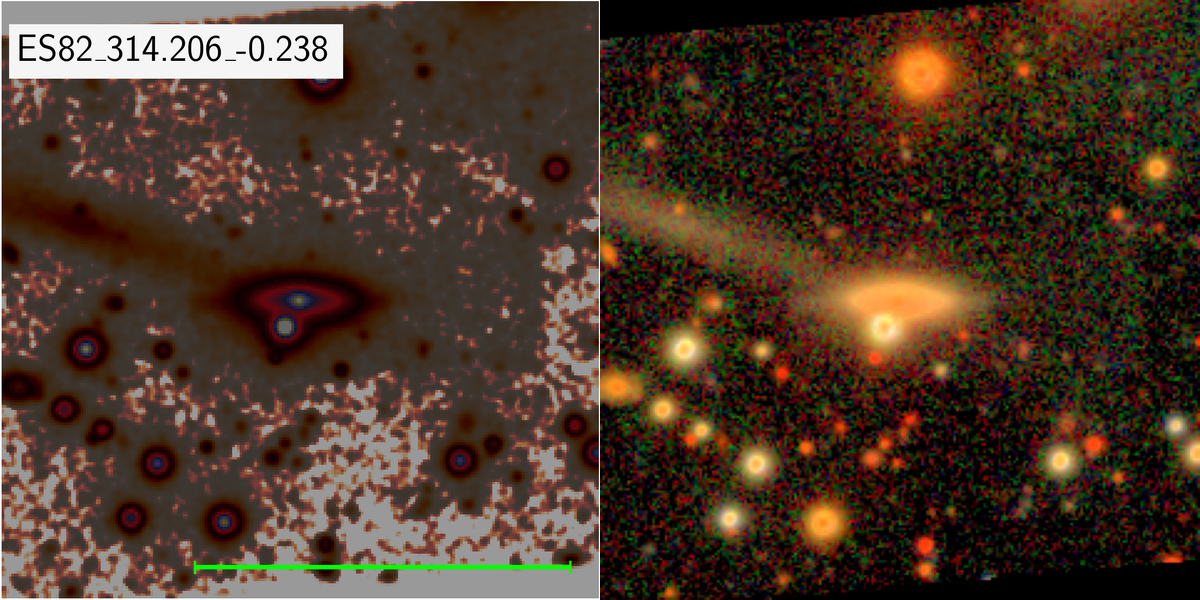
\includegraphics[width=.5\textwidth]{images/526.png}\hfill
    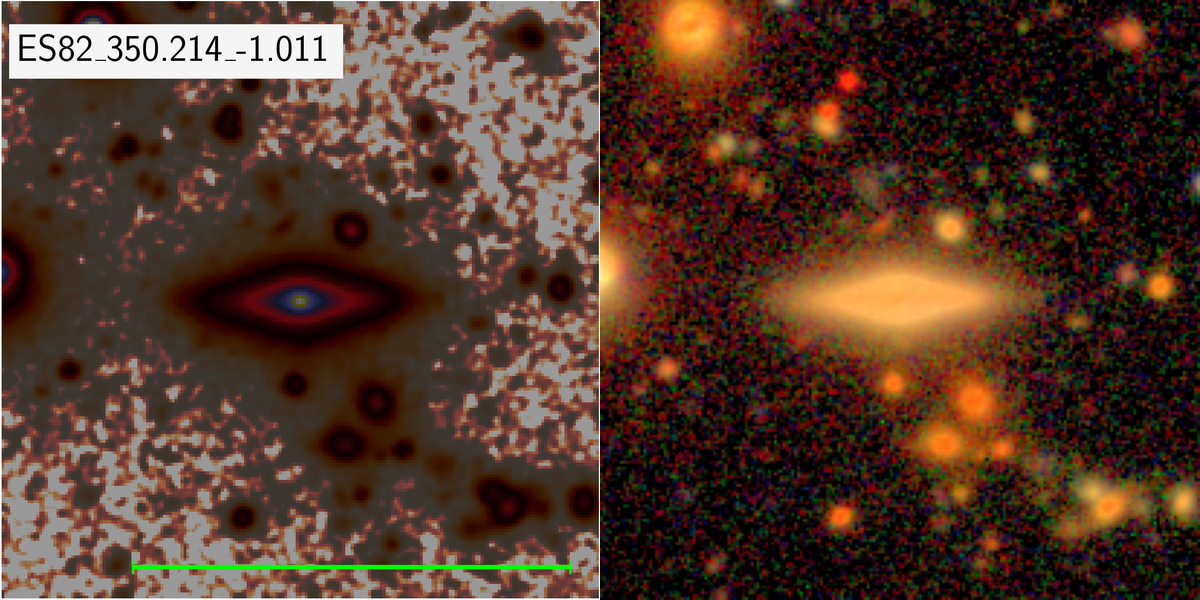
\includegraphics[width=.5\textwidth]{images/777.png}\hfill
    \caption{Примеры галактик с хвостами. Левая панель -- суммарное изображение галактики, правая панель -- цветное RGB изображение.}\label{fig:tails}
\end{figure}

\begin{figure}[ht]

    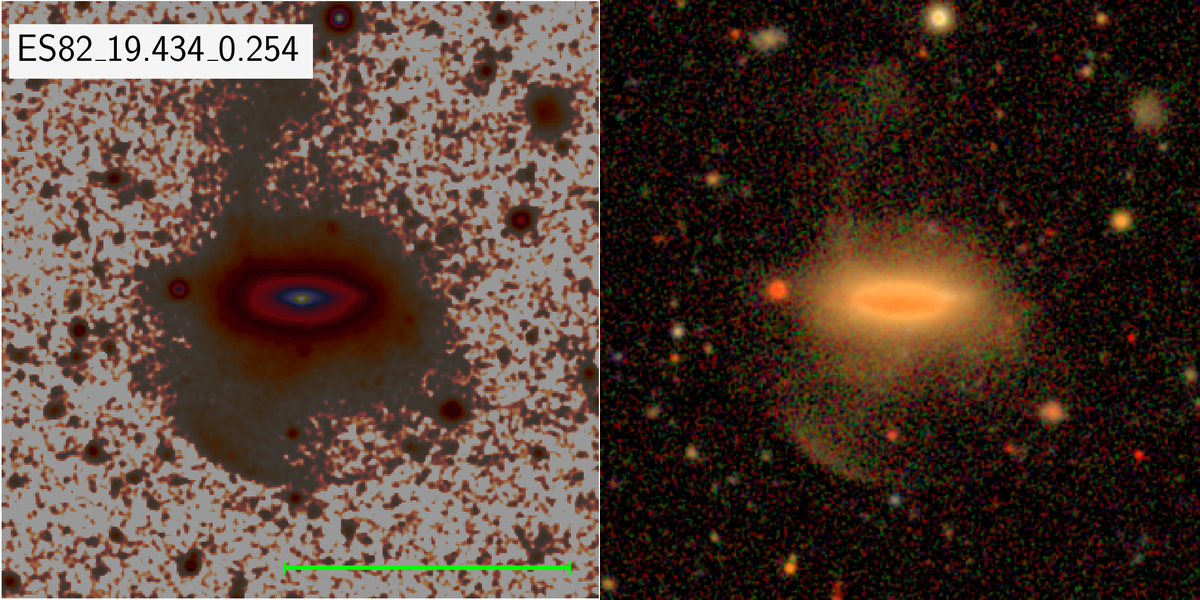
\includegraphics[width=.5\textwidth]{images/222.png}\hfill
    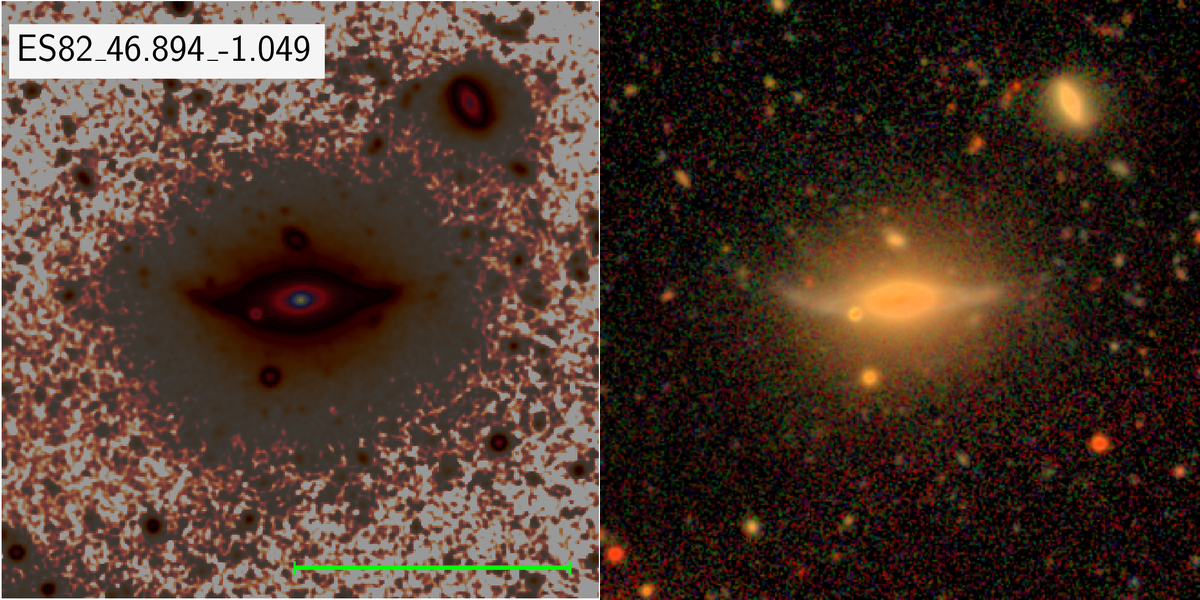
\includegraphics[width=.5\textwidth]{images/424.png}\hfill

    \caption{Примеры галактик с оболочками. Левая панель -- суммарное изображение галактики, правая панель -- цветное RGB изображение.}\label{fig:shells}
\end{figure}

\begin{figure}[ht]

    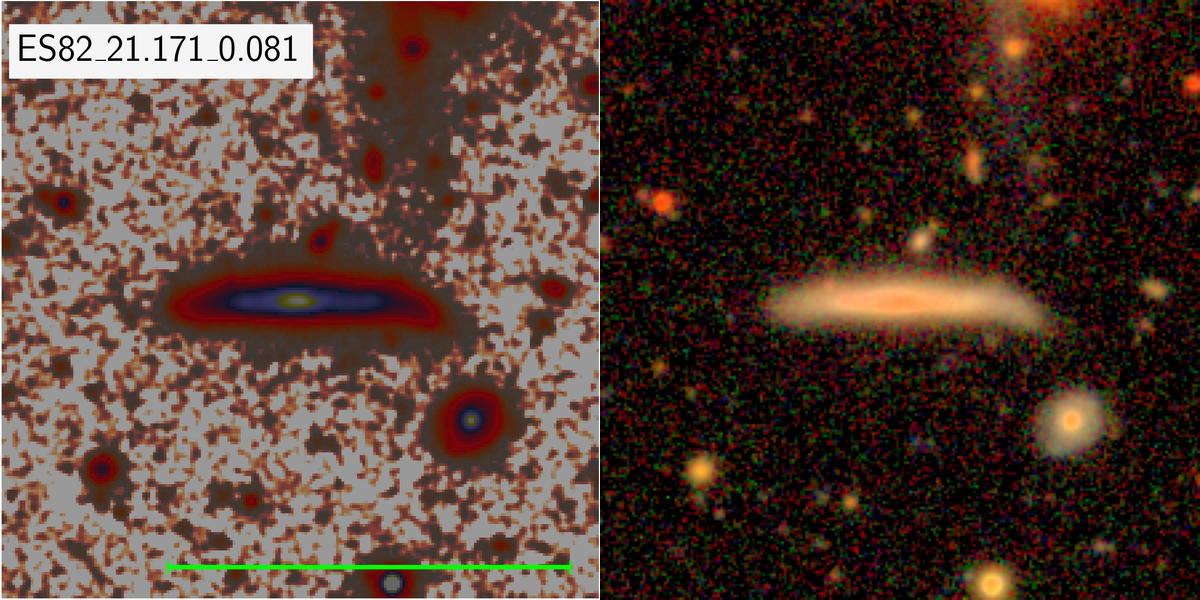
\includegraphics[width=.5\textwidth]{images/247.png}\hfill
    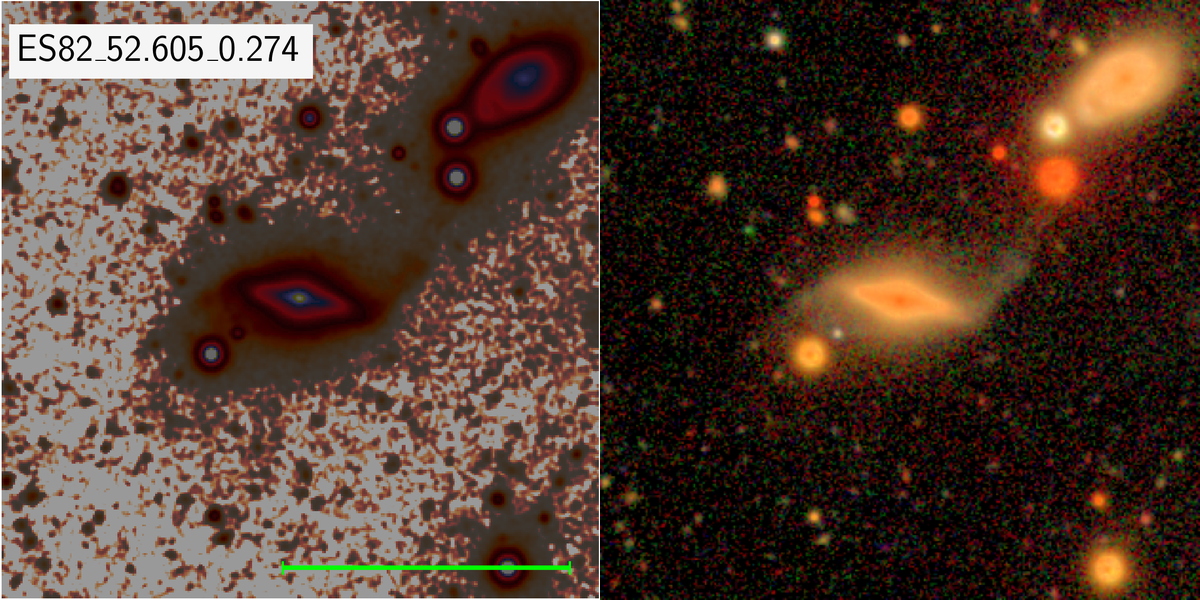
\includegraphics[width=.5\textwidth]{images/471.png}\hfill
    \caption{Примеры галактик с мостами. Левая панель -- суммарное изображение галактики, правая панель -- цветное RGB изображение.}\label{fig:bridges}
\end{figure}

\begin{figure}[ht]

    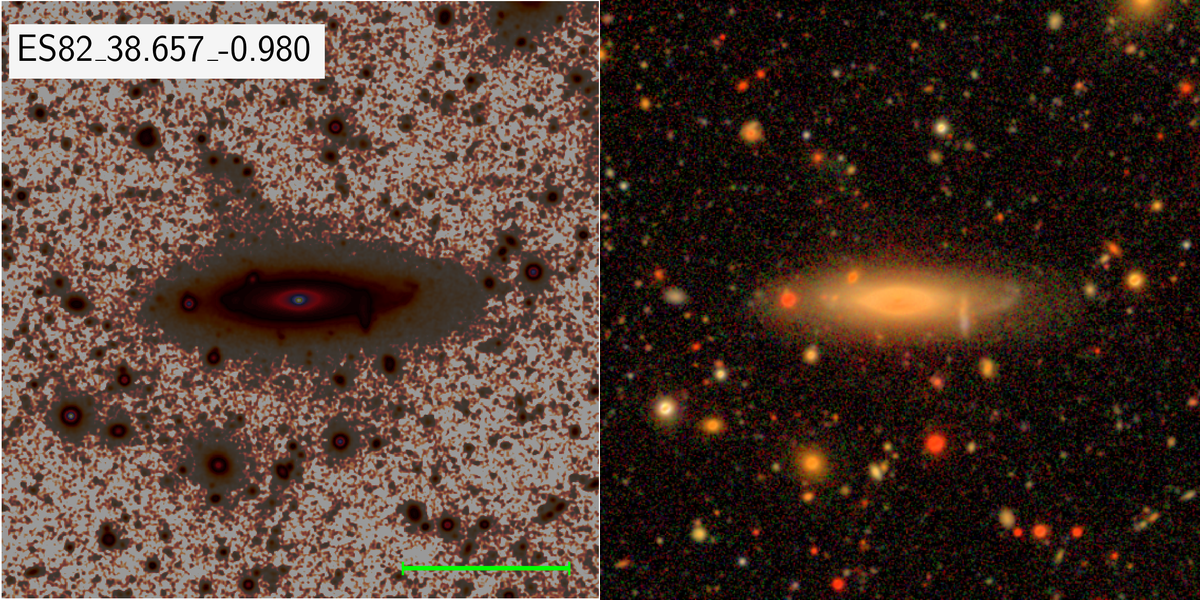
\includegraphics[width=.5\textwidth]{images/52.png}\hfill
    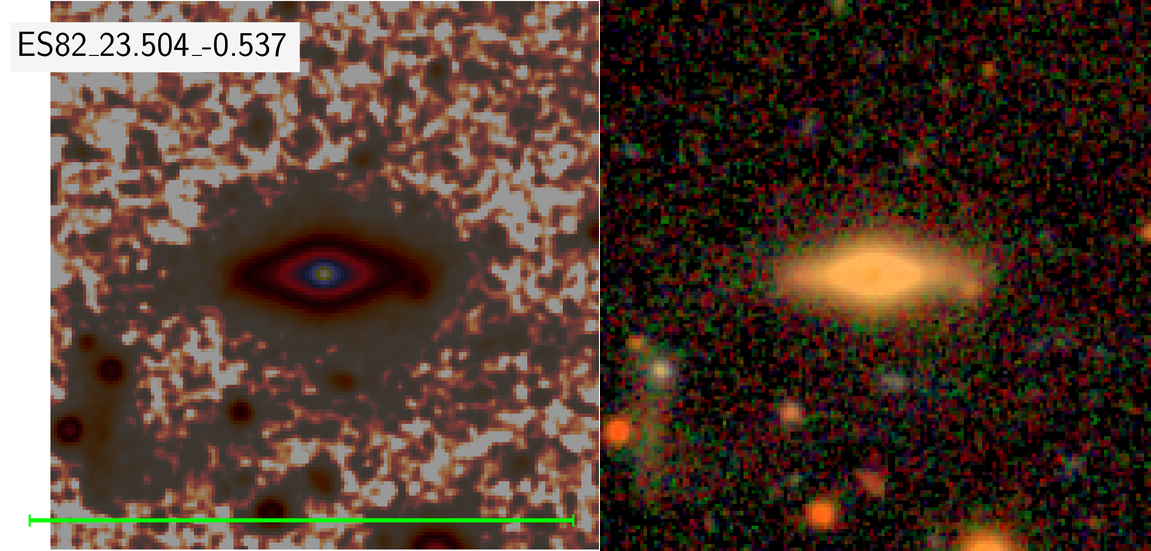
\includegraphics[width=.5\textwidth]{images/262.png}\hfill

    \caption{Примеры галактик с арками. Левая панель -- суммарное изображение галактики, правая панель -- цветное RGB изображение.}\label{fig:arcs}
\end{figure}

\begin{figure}[ht]

    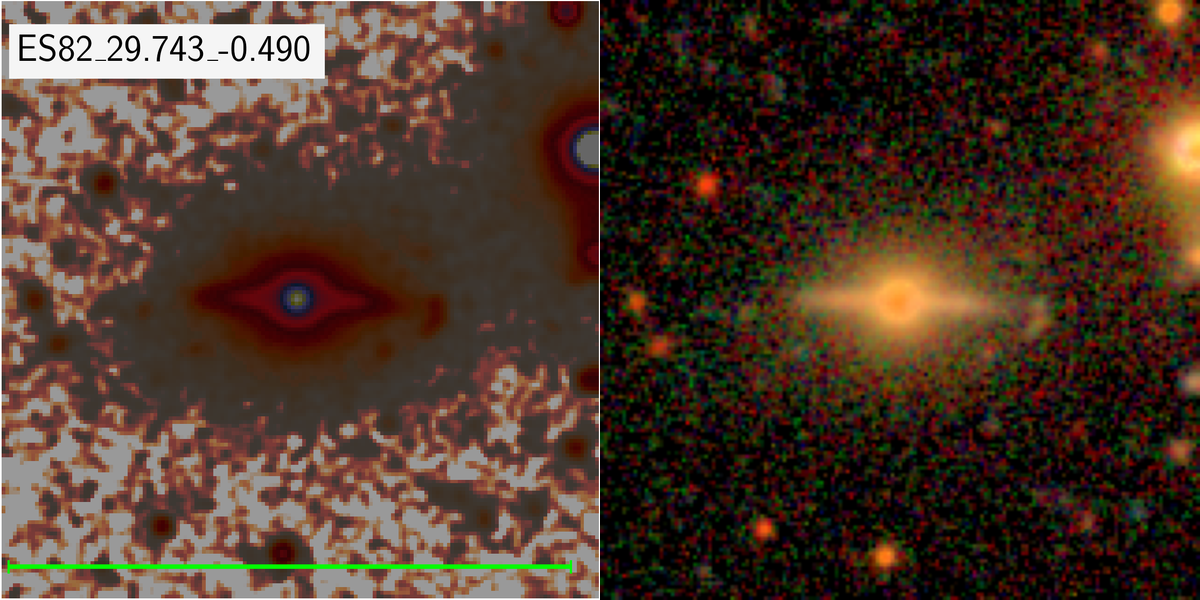
\includegraphics[height=.14\textheight]{images/307.png}\hfill
    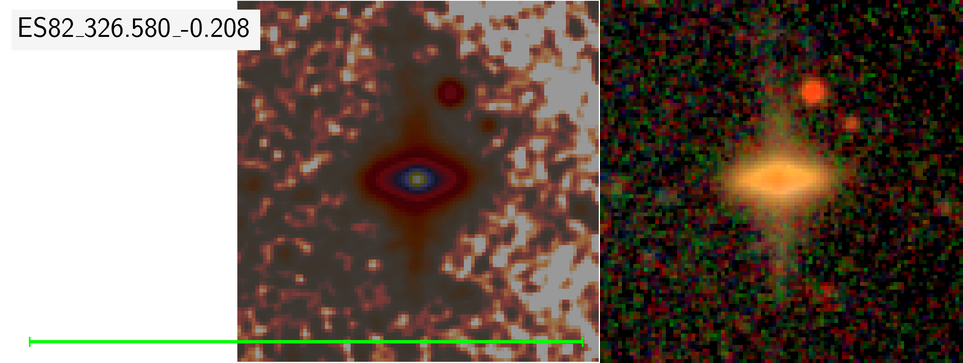
\includegraphics[height=.14\textheight]{images/627.png}\hfill

    \caption{Примеры галактик с полярными кольцами. Левая панель -- суммарное изображение галактики, правая панель -- цветное RGB изображение.}\label{fig:rings}
\end{figure}

\begin{figure}[ht]

    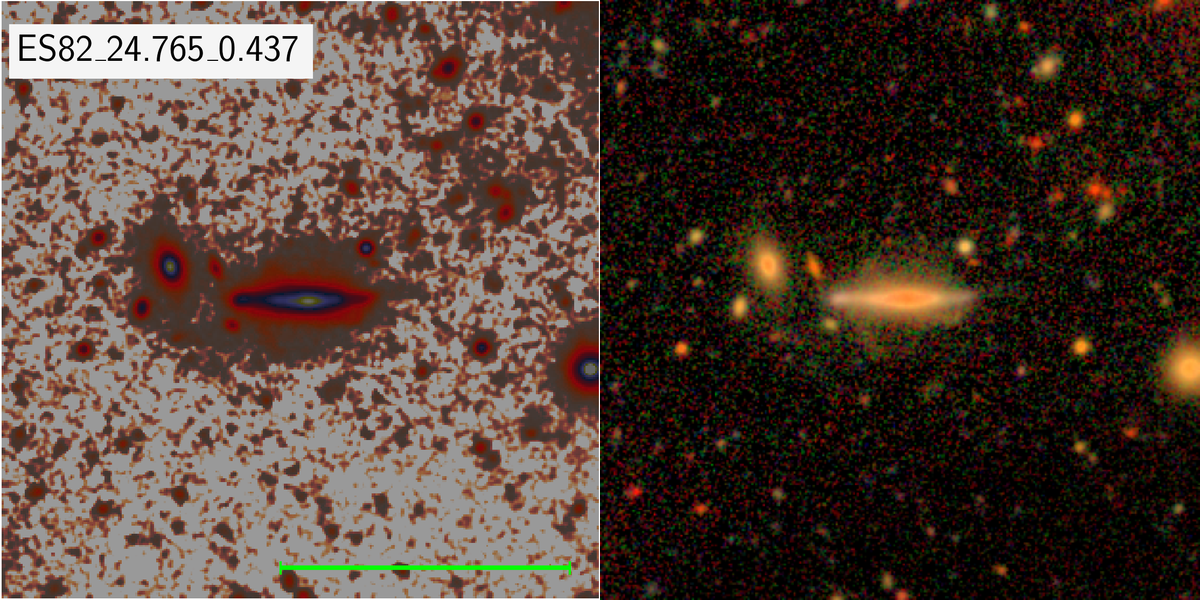
\includegraphics[width=.5\textwidth]{images/270.png}\hfill
    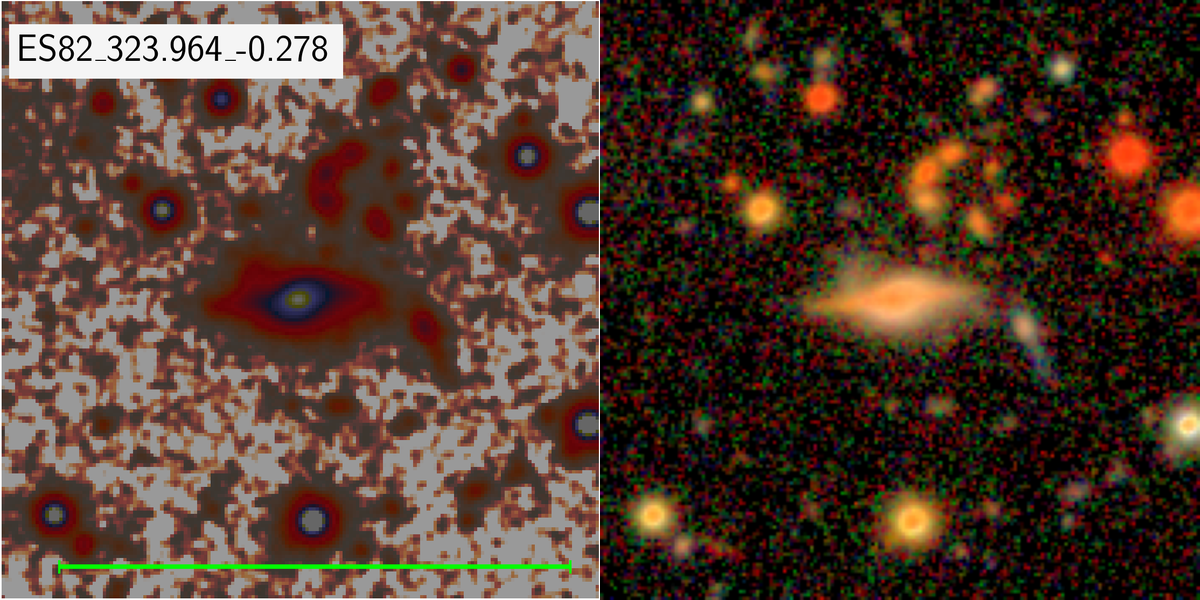
\includegraphics[width=.5\textwidth]{images/602.png}\hfill

    \caption{Примеры галактик с остатками спутников. Левая панель -- суммарное изображение галактики, правая панель -- цветное RGB изображение.}\label{fig:debris}
\end{figure}

\begin{figure}[ht]

    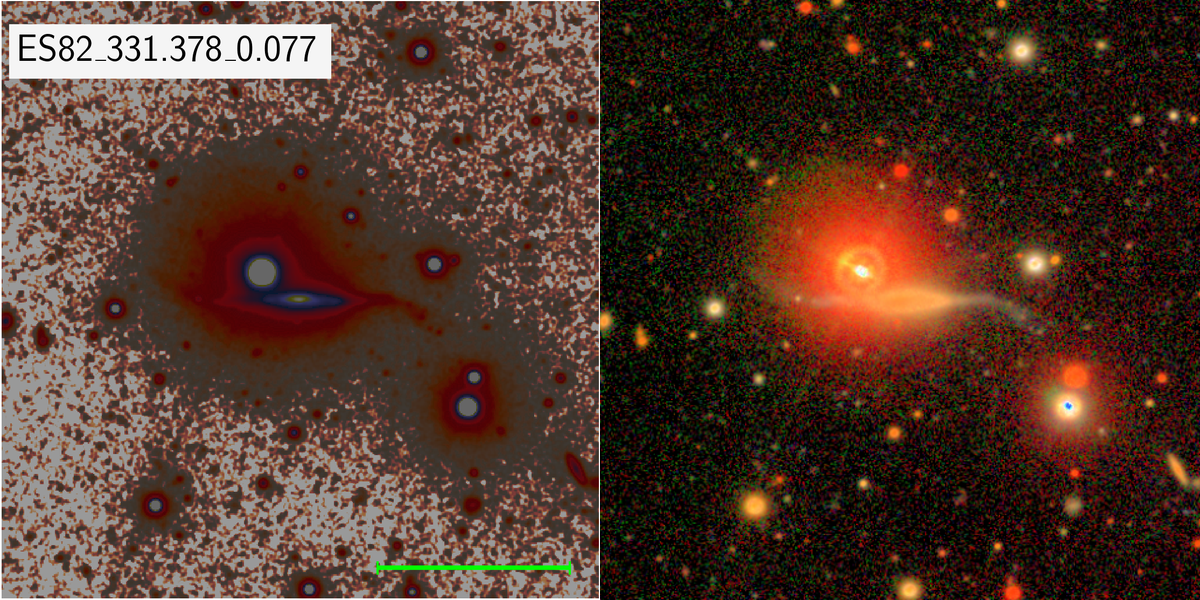
\includegraphics[width=.5\textwidth]{images/11.png}\hfill
    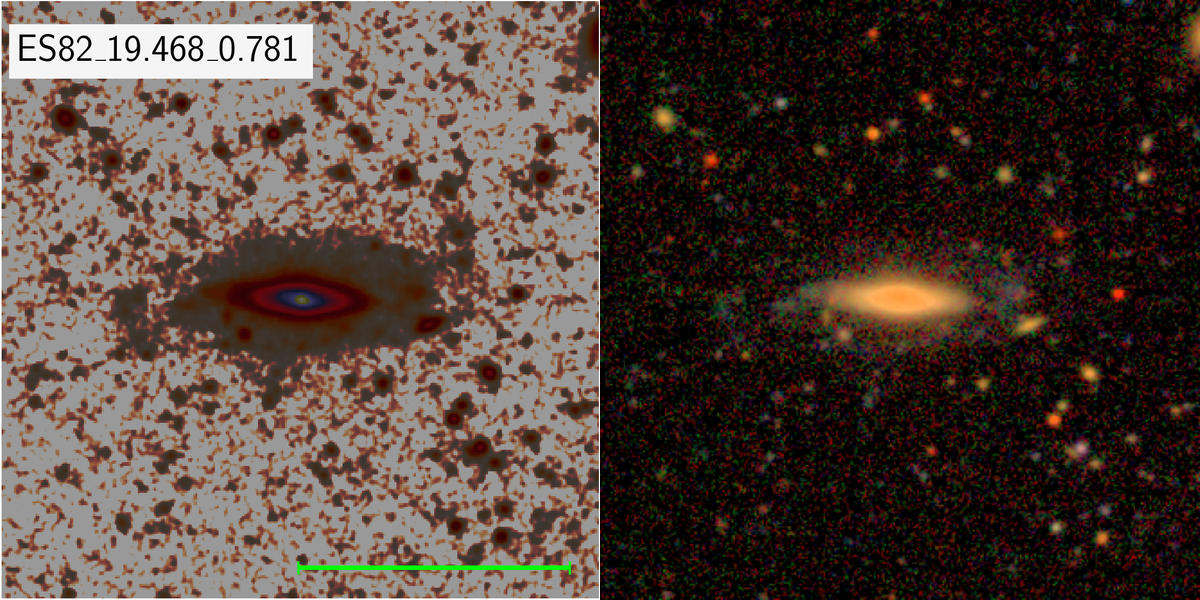
\includegraphics[width=.5\textwidth]{images/224.png}\hfill

    \caption{Примеры галактик с изгибами диска. Левая панель -- суммарное изображение галактики, правая панель -- цветное RGB изображение.}\label{fig:warp}
\end{figure}

\begin{figure}[ht]

    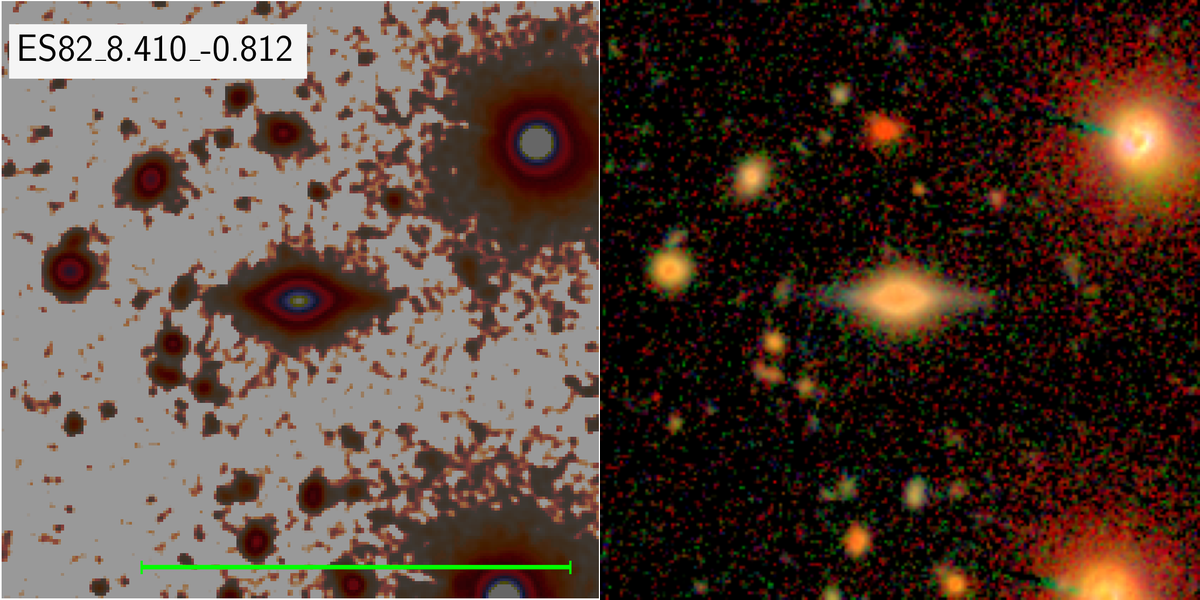
\includegraphics[width=.5\textwidth]{images/139.png}\hfill
    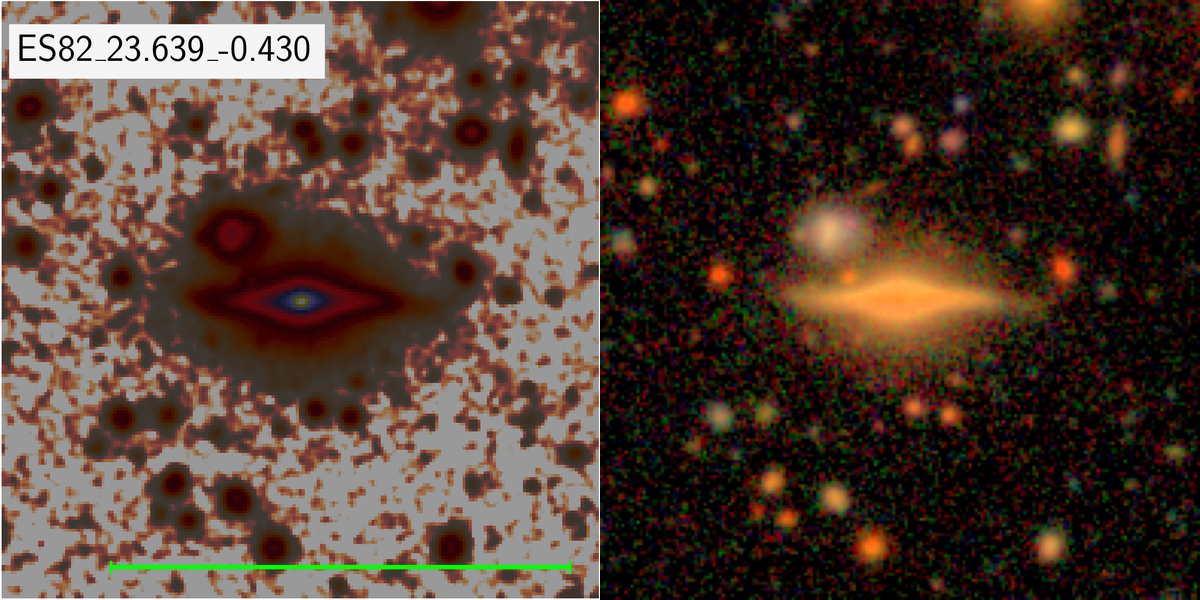
\includegraphics[width=.5\textwidth]{images/263.png}\hfill

    \caption{Примеры галактик с балджем. Левая панель -- суммарное изображение галактики, правая панель -- цветное RGB изображение.}\label{fig:bulge}
\end{figure}

\begin{figure}[ht]

    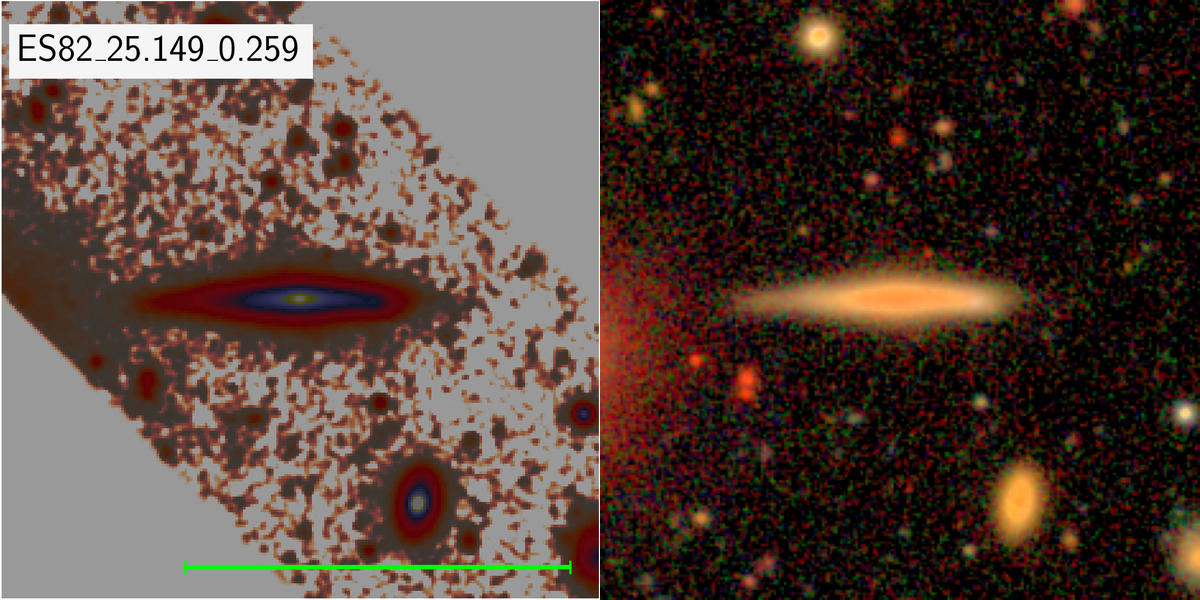
\includegraphics[width=.5\textwidth]{images/45.png}\hfill
    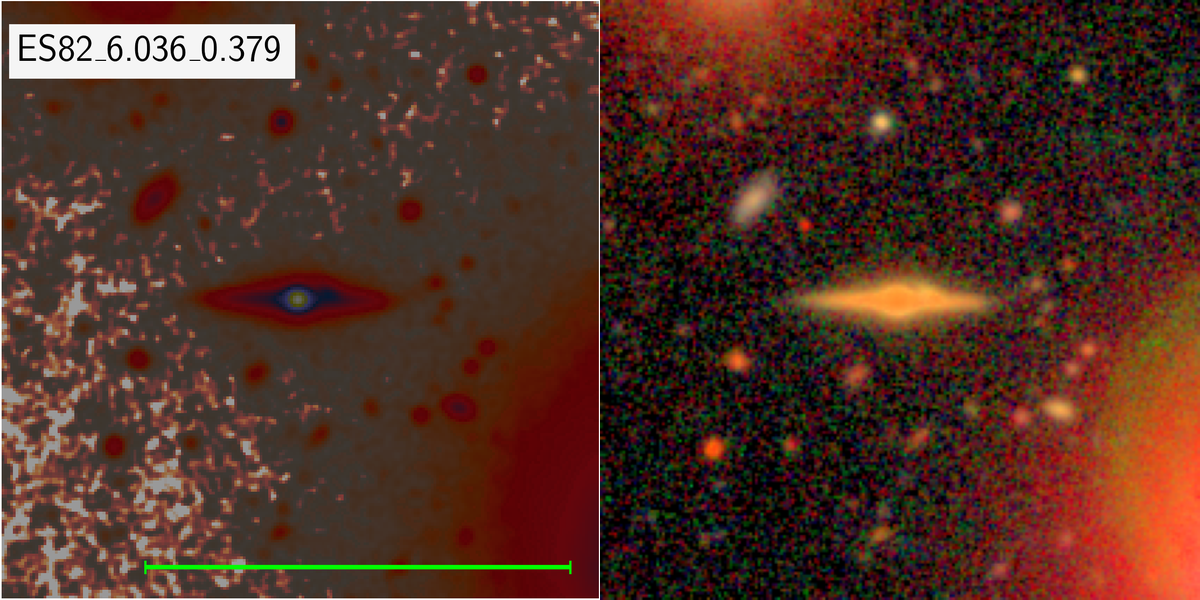
\includegraphics[width=.5\textwidth]{images/118.png}\hfill

    \caption{Примеры галактик с кособокими звездными дисками. Левая панель -- суммарное изображение галактики, правая панель -- цветное RGB изображение.}\label{fig:lopsided}
\end{figure}

\section{Статистика проклассифицированных структур}

Один из важных результатов данной работы, это статистика по распределению различных приливных структур, а также структурных особенностей галактик выборки.

Суммарно, приливные структуры низкой поверхностной яркости наблюдаются у 43 объектов. 
Количество галактик с различными приливными LSB структурами:
\begin{enumerate}
    \item Хвосты -- 6
    \item Мосты -- 8
    \item Арки -- 7
    \item Полярные кольца -- 2
    \item Остатки спутников -- 9
    \item Оболочки  -- 15
\end{enumerate}

Также собрана статистика по наблюдаемым структурам низкой поверхностной яркости, не являющихся прилиливными.
Всего галактик, обладающих подобными структурами – 86. Подробнее  по каждой структуре:
\begin{enumerate}
    \item Балджи (толстые коробкоподобные балджи, уплощенные балджеподобные структуры, полярные балджи)  --  36
    \item Изгибы диска  --  58
    \item Кособокость  --  10
    \item Другие (структурные особенности по типу спиралей)  --  5
\end{enumerate}

Основной результат данного раздела заключается в том, что несмотря на большую выборку галактик и глубину изображений, относительное количество объектов, обладающих приливными структурами, меньше ожидаемого. Взаимодействующие галактики, это распространенное явление во Вселенной, что мы можем наблюдать даже на примере нашей галактики Млечный Путь. 


\section{Фотометрическая декомпозиция}
На данном этапе производится детальный анализ изображений видимых с ребра галактик в полосе Stripe 82, с целью оценки вертикальных и радиальных масштабов их звездных дисков.

Для описания распределения яркости вдоль направления малой оси галактики, видимой с ребра, обычно применяется модель самогравитирующего изотермического слоя \cite{1981A&A....95..105V}, для которого \ref{eq:sech}:
\begin{equation}
I(z) = I_0\sech^2(z/z_0)
\label{eq:sech}
\end{equation}
где $z_0$ -- вертикальный масштаб, то есть масштаб распределения яркости вдоль перпендикулярного к плоскости диска направления (вдоль координаты z). В рамках этой модели вертикальный масштаб связан с вертикальной
дисперсией скоростей звезд и их объемной и поверхностной плотностью. 
Вблизи от плоскости галактики $(z/z_0 \ll 1)$: $\sech^2(z/z_0) = exp(-z^2/z_0^2)$.
Вдали от плоскости $(z/z_0 \gg 1)$: $\sech^2(z/z_0) = 4exp(-2z/z_0^2) $.
Можно ввести еще одну формулу \ref{eq:exp} экспоненциального закона, совпадающую с \ref{eq:sech} в случаях $z/z_0 \ll 1$ и $z/z_0 \gg 1$:
\begin{equation}
    I(z) = exp(-|z|/h_z),
    \label{eq:exp}
\end{equation}
где $h_z$ -- экспоненциальный масштаб распределения яркости вдоль перпендикулярного к диску направления (вдоль координаты z). Формулы \ref{eq:sech} и \ref{eq:exp} связаны через соотношение $z_0 = 2h_z$.
Наблюдения показывают, что для некоторых галактик формула \ref{eq:exp} вполне адекватно описывает наблюдаемое распределение яркости. 

В свою очередь, распределение яркости в радиальном направлении в диске спиральной галактики, видимой плашмя, может быть хорошо описано экспоненциальным законом с радиальным масштабом $h_r$ \cite{1959HDP....53..275D} \cite{1940BHarO.914....9P}:
\begin{equation}
    I(r) = I_0exp(-r/h_r)
    \label{eq:radexp}
\end{equation}
Таким образом, $h_z$ и $h_r$ – вертикальный и радиальный экспоненциальные масштабы диска. Они могут быть использованы для описания глобальной фотометрической структуры галактик. В данном разделе получение и анализ этих параметров является основной задачей. 

Мы можем совместить формулы распределения поверхностной яркости в радиальном и вертикальном направлениях. Модель диска спиральной галактики в этом случае будет выражаться следующей формулой:
\begin{equation}
    I(r,z) = I_0e^{-r/h}sech^2{z/z_0}
    \label{eq: combined}
\end{equation}
Здесь радиальный масштаб обозначается как \textit{h}, а вертикальный – как $z_0$. Такие обозначения будут применены и для следующих формул данного раздела.
В работе van der Kruit P.C., Searle L. \cite{1981A&A....95..105V} вычислена поверхностная яркость с законом распределения \ref{eq: combined} для спиральной галактики, наблюдаемой с ребра:
\begin{equation}
    \mu(r,z) = \mu(0,0)(r/h)K_1(r/h)sech^2(z/z_0)
    \label{vanderkruit}
\end{equation}
где $K_1$ -- модифицированная функция Бесселя первого порядка. Центральная поверхностная яркость выражается следующим образом:
\begin{equation}
    \mu(0,0) = 2hL_0,
\end{equation}
где $L_0$ -- центральная поверхностная яркость.
Позднее в работе того же автора \cite{1988A&A...192..117V} было предложено использовать более общий закон для описания распределения плотности светящегося вещества в галактике вдоль координаты z:
\begin{equation}
    \rho(z) = 2^{-2/n}\rho_0\sech^{2/n}(nz/(2z_0))\hspace{2em}(n>0), 
    \label{eq:new_law}
\end{equation}
в котором степень $2/n$ регулирует форму распределения.
при $n = 1$ формула \ref{eq:new_law} переходит в модель изотермического слоя (формула \ref{eq:sech}), при $n = \infty$ в экспоненциальный закон (формула \ref{eq:exp}).
Отсюда, согласно \cite{1988A&A...192..117V}, получается следующая формула распределения поверхностной яркости для видимой с ребра галактики:
\begin{equation}
    I(r,z) = \mu(0,0)(r/h)K_1(r/h)sech^{2/n}(nz/(2z_0))
    \label{eq:final_law}
\end{equation}

Важно отметить, что в процессе выполнения фотометрической декомпозиции был зафиксирован параметр $n$, он был принят равным значению $n = 100$. Тогда, согласно формуле \ref{eq:final_law}, $\sech^{2/n}(nz/(2z_0)) \approx exp(z/z_0)$. То есть распределение яркости всех галактик вдоль вертикального направления было аппроксимировано простым экспоненциальным законом.

Для получения начального приближения вертикального и радиального масштабов диска была выполнена одномерная фотометрическая декомпозиция компонент диска и балджа. Для этого были модифицированы python скрипты, подготовленные научным руководителем, Савченко С.С. \footnote{https://bitbucket.org/latrop/decomposer/src/master/}. Используя результаты одномерной декомпозиции в качестве входных параметров была осуществлена двумерная декомпозиция.
Порядок выполнения фотометрической декомпозиции был следующий:
\begin{enumerate}
    \item Изначально была составлена "золотая"$\,$         выборка галактик, наблюдаемых точно с ребра. Это определялось, например, по расположению пылевой полосы. Также критериями отбора галактик являлось наличие регулярной структуры без особенностей, отсутствие ярких источников в близкой окрестности галактики (чтобы само тело галактики не сильно перекрывалось другими источниками и не было ярких звёзд поблизости). Полученная выборка включает 73 объекта.
    \item Перед выполнением одномерной декомпозиции были заранее подготовлены обрезанные изображения галактик (со стороной изображения 3 размера большой полуоси по горизонтали, и малой оси по вертикали), соразмерные файлы масок, файлы весов, файлы psf, помогающие учитывать влияние оптической системы и атмосферной турбулентности.
    \item Для выполнения декомпозиции достаточно указать номер галактики в выборке в качестве ключа при запуске скрипта. В процессе работы программы для каждой галактики было построено 2 модели: первая -- простая модель, использующая функцию \ref{eq:final_law} (соответсвующая функция в Imfit -- EdgeOnDisk) и описывающая галактику как объект, расположенный точно с ребра. Во второй модели добавляется компонента балджа, аппроксимируемая функцией Серсика:
    \begin{equation}
        I(a) = I_eexp\Bigg\{-b_n\Bigg[\bigg(\frac{a}{r_e}^{1/n}-1\bigg)\Bigg]\Bigg\},
        \label{Sersic}
    \end{equation}
    где $I_e$ -- поверхностная яркость на эффективном радиусе $r_e$,  n -- индекс Серсика, значение параметра $b_n$ формально задает решение трансцендентного выражения $\Gamma(2n) = 2\gamma(2n, b_n)$. Здесь $\Gamma(a)$ -- гамма-функция, а $\gamma(a,x)$ -- неполная гамма-функция. 
    \item Для каждой из двух моделей было автоматически посчитано значение BIC (the Bayesian information criterion), расчитываемое по формуле: $BIC = -2\ln\textit{L} + k\ln(n)$, где \textit{L} -- максимальное значение функции правдоподобия наблюдаемой выборки с известным числом параметров, k -- количество свободных параметров, n -- количество незамаскрированных пикселей на изображении. Выбиралась та модель, значение BIC для которой наименьшее. 
    \item На выходе мы имеем конфиругационный файл Imfit, в котором описаны 7 параметров диска: 
    
    \begin{tabular}{p{40mm}p{5mm}p{90mm}}
    
    \texttt{X0} & -- & координата центра по оси X изображения  \\
    \texttt{Y0} & -- & координата центра по оси X изображения \\
    \texttt{EdgeOnDisk} & -- &функция для аппроксимации \\
    \texttt{PA} & -- &позиционный угол (угол между осью Y изображения и осью координаты r, отсчитываемый против часовой стрелки  \\
    \texttt{$L\_0$} & -- &центральная плотность светимости $L_0$ \\
    \texttt{h} & -- & радиальный масштаб $h$ \\
    \texttt{n} & -- & индекс Серсика $n$ \\
    \texttt{$z\_0$} & -- & вертикальный масштаб $z_0$
    \end{tabular}

    \item Следующий выполненный этап -- двумерная декомпозиция в Imfit\cite{2015ApJ...799..226E}. На вход программы осуществлялась подача изображения галактики, конфигурационного файла с комбинацией двумерных функций (результат одномерной декомпозиции), которые должны аппроксимировать распределение поверхностной яркости при декомпозиции, также файлы с маской и весами, psf-изображение.
    \item Построены модельные изображения галактик, описываемых комбинацией двумерных функций с заданными параметрами.
    \item Получены разностные изображения и вычислена статистическая разница реального и модельного изображений галактики (по критерию $\chi^2$ ) c применением информации о достоверности значений
в пикселях, содержащейся в изображениях масок и весов.
    \item Выполнена корректировка параметров модельных двумерных функций в сторону уменьшения статистической разницы $\chi^2$ методом градиентного спуска.
    \item Построены срезы вдоль большой и малой полуоси галактики в сравнении с моделями, описываемыми полученными в процессе двумерной декомпозиции параметрами (Рис. \ref{fig:slices}). Получены изображения моделей и их разностей с изображениями реальных галактик (Рис. \ref{fig:models}).
    
\end{enumerate}

\begin{figure}[p]
    \centering
    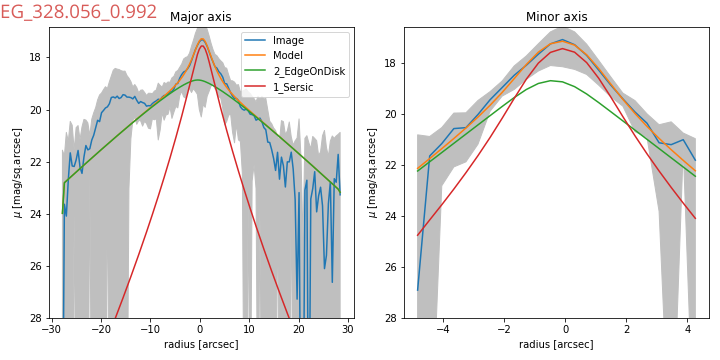
\includegraphics[width=.9\textwidth]{plot_results/4.png}\hfill\\
    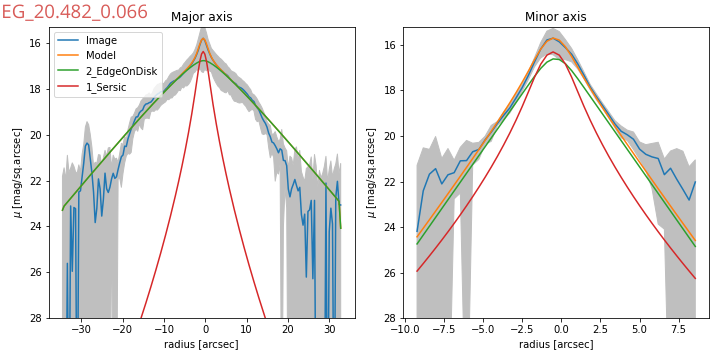
\includegraphics[width=.9\textwidth]{plot_results/6.png}\hfill\\
    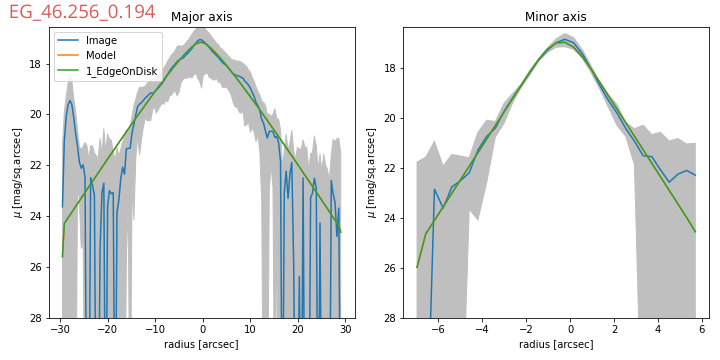
\includegraphics[width=.9\textwidth]{plot_results/5.png}\hfill\\

    \caption{Примеры полученных результатов двумерной декомпозиции: левая панель -- разрез вдоль большой полуоси галактики, правая панель -- разрез вдоль малой полуоси галактики. Зеленым цветом изображена модельная компонента диска, красным -- компонента балджа (если имеется), желтым -- сумма двух компонент. }\label{fig:slices}
\end{figure}

\begin{figure}[p]
    \centering
    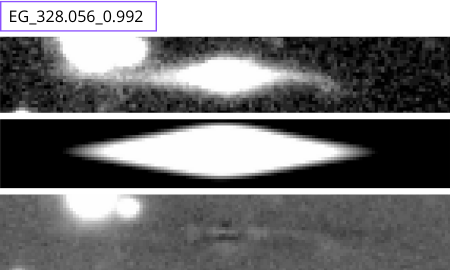
\includegraphics[width=.7\textwidth]{plot_results/1.png}\hfill\\
    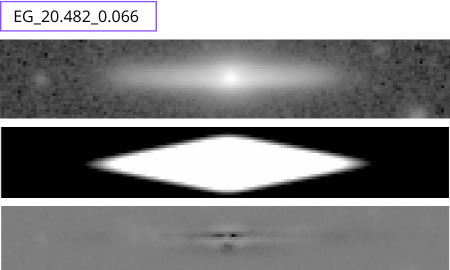
\includegraphics[width=.7\textwidth]{plot_results/2.png}\hfill\\
    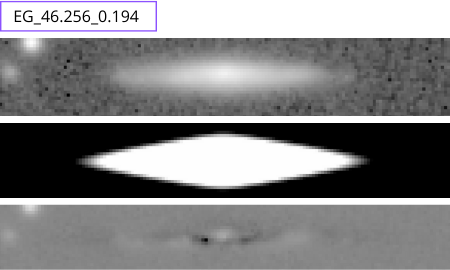
\includegraphics[width=.7\textwidth]{plot_results/3.png}\hfill\\

    \caption{Примеры полученных результатов двумерной декомпозиции: левая панель -- изображение реальной галактики, средняя панель -- модель, правая панель -- разность изображения реальной галактики и модели.  }\label{fig:models}
\end{figure}
\section{Результаты декомпозиции}
В процессе анализа результатов двумерной декомпозиции был сделан вывод о том, что не для всех галактик "золотой"\textrm{ } выборки полученные модели являются достоверным приближением распределения их поверхностной яркости. Некоторые галактики требуют введения более сложных моделей (учитывающих изломы диска  или же угол наклона относительно луча зрения). Из выборки  галактик, с которыми производилась фотометрическая декомпозиция (73 галактики), 51 галактика имеет адекватно построеную модель, остальные требуют введения более сложных 3D моделей (все дальнейшие шаги производились именно с подвыборкой галактик, имеющих хорошие результаты фотометрической декомпозиции -- 51 галактика). 

Прежде, чем переходить к анализу, мы решили сравнить звездные величины модельных галактик со звездными величинами из базы данных SDSS\footnote{\url{http://skyserver.sdss.org/DR16/en/tools/crossid/crossid.aspx}}, таким образом, мы сможем сделать выводы о качестве выполненной декомпозиции. В таблице \ref{tab:mags} приведены видимые звездные величины построенных модельных галактик и звездные величины реальных галактик выборки, полученные из базы данных SDSS в фильтре r. 
\begin{longtable}{|l|l|l|l|l|l|}
\caption{Значения видимых звездных величин из базы данных SDSS и модельных (SDSS фильтр r). Первый столбец -- номер галактики, второй -- звездная величина реальной галактики из базы данных SDSS, третий -- модельная звездная величина, посчитанная по результатам одномерной декомпозиции, четвертый -- модельная звездная величина, посчитанная по результатам двумерной декомпозиции, пятые и шестой -- модули разностей реальных и модельных звездных величин.} \label{tab:mags}  \\ \hline
 N & $m_r(SDSS)$ & $m_r(1d)$ & $m_r(2d)$  & |$m_r(SDSS)$-$m_r(1d)$|  & |$m_r(SDSS)$-$m_r(2d)$|\\\hline\hline

        1 & 18.021 & 18.551 & 18.063 & 0.53 & 0.041 \\ 
        2 & 17.891 & 20.49 & 17.854 & 2.599 & 0.038 \\ 
        3 & 16.538 & 19.218 & 16.424 & 2.68 & 0.114 \\ 
        4 & 16.398 & 16.898 & 15.625 & 0.5 & 0.773 \\ 
        5 & 16.903 & 19.992 & 16.815 & 3.089 & 0.088 \\ 
        6 & 17.572 & 20.234 & 17.269 & 2.662 & 0.303 \\ 
        7 & 16.456 & 16.807 & 16.657 & 0.351 & 0.201 \\ 
        8 & 17.709 & 17.652 & 17.441 & 0.057 & 0.269 \\ 
        9 & 17.099 & 19.876 & 17.057 & 2.777 & 0.041 \\ 
        10 & 17.208 & 17.414 & 17.359 & 0.206 & 0.151 \\ 
        11 & 18.102 & 20.861 & 18.078 & 2.76 & 0.024 \\ 
        12 & 16.308 & 16.339 & 16.284 & 0.03 & 0.025 \\ 
        13 & 16.016 & 19.056 & 15.89 & 3.039 & 0.127 \\ 
        14 & 17.021 & 19.87 & 16.915 & 2.849 & 0.106 \\ 
        15 & 16.36 & 18.872 & 16.272 & 2.512 & 0.088 \\ 
        16 & 15.829 & 15.561 & 15.259 & 0.269 & 0.57 \\ 
        17 & 17.435 & 19.811 & 17.357 & 2.376 & 0.078 \\ 
        18 & 15.475 & 18.257 & 15.85 & 2.782 & 0.375 \\ 
        19 & 17.788 & 19.632 & 17.598 & 1.844 & 0.189 \\ 
        20 & 16.917 & 19.691 & 16.907 & 2.775 & 0.009 \\ 
        21 & 17.113 & 19.661 & 17.089 & 2.548 & 0.024 \\ 
        22 & 16.217 & 16.826 & 16.49 & 0.609 & 0.272 \\ 
        23 & 17.357 & 18.164 & 17.504 & 0.807 & 0.147 \\ 
        24 & 15.843 & 16.652 & 16.006 & 0.809 & 0.163 \\ 
        25 & 16.973 & 19.09 & 16.818 & 2.118 & 0.154 \\ 
        26 & 17.258 & 16.875 & 17.056 & 0.383 & 0.202 \\ 
        27 & 16.851 & 18.854 & 16.787 & 2.003 & 0.064 \\ 
        28 & 15.43 & 14.465 & 15.273 & 0.965 & 0.157 \\ 
        29 & 17.639 & 17.894 & 17.528 & 0.255 & 0.111 \\ 
        30 & 17.562 & 20.137 & 17.554 & 2.575 & 0.008 \\ 
        31 & 17.119 & 17.582 & 16.891 & 0.463 & 0.228 \\ 
        32 & 16.667 & 17.167 & 16.502 & 0.5 & 0.165 \\ 
        33 & 16.659 & 20.212 & 16.422 & 3.553 & 0.237 \\ 
        34 & 15.283 & 15.288 & 15.393 & 0.006 & 0.111 \\ 
        35 & 16.256 & 17.112 & 16.497 & 0.856 & 0.241 \\ 
        36 & 14.617 & 17.11 & 14.458 & 2.493 & 0.158 \\ 
        37 & 16.345 & 16.184 & 16.038 & 0.16 & 0.307 \\ 
        38 & 17.744 & 20.385 & 17.628 & 2.641 & 0.115 \\ 
        39 & 16.393 & 16.385 & 16.529 & 0.008 & 0.136 \\ 
        40 & 16.304 & 16.034 & 16.473 & 0.27 & 0.169 \\ 
        41 & 17.577 & 18.195 & 17.538 & 0.618 & 0.04 \\ 
        42 & 17.496 & 18.45 & 17.054 & 0.954 & 0.442 \\ 
        43 & 17.27 & 17.198 & 17.247 & 0.073 & 0.024 \\ 
        44 & 16.78 & 17.194 & 16.722 & 0.413 & 0.058 \\ 
        45 & 15.82 & 16.846 & 15.413 & 1.026 & 0.407 \\ 
        46 & 16.936 & 17.844 & 16.723 & 0.908 & 0.213 \\ 
        47 & 16.727 & 19.026 & 16.64 & 2.299 & 0.087 \\ 
        48 & 16.826 & 17.562 & 17.041 & 0.737 & 0.216 \\ 
        49 & 15.766 & 18.25 & 15.604 & 2.484 & 0.162 \\ 
        50 & 17.561 & 18.829 & 17.281 & 1.268 & 0.28 \\ 
        51 & 15.966 & 16.98 & 15.694 & 1.014 & 0.272 \\ \hline
\end{longtable} Обращаем внимание на то, что результаты одномерной декомпозиции значительно хуже результатов двумерной. В то время, как модельная звездная величина, полученная по результатам двумерной декомпозиции отличается от реальной (SDSS) в десятых или сотых,  разница модельной звездной величины, полученной по результатам одномерной декомпозиции с реальной (SDSS) в некоторых случаях отличается на 2 или 3 звездные величины. Таким образом, результаты двумерной декомпозиции более точные, в дальнейшем мы будем опираться на них, но и анализ одномерной декомпозиции также будет осуществлен для сравнения.

Возвращаясь к масштабным параметрам, в таблице \ref{tab:tab3} приведены параметры (радиальный и вертикальный масштабы) для галактик выборки.
% Также на основе результатов декомпозиции были построены различные графики зависимостей:
\begin{longtable}{|l|l|l|l|l|l|l|l|l|}
\caption{Масштабные параметры галактик выборки, полученные в результате декомпозиции. Столбцы \textit{1d} содержат в себе информацию по одномерной декомпозиции. Столбцы \textit{2d} - информацию по двумерной декомпозиции. $h$ и $h_z$ - радиальный и вертикальные экспоненциальные масштабы дисков.} \label{tab:tab3}  \\ \hline
 N & h (1d) & h (2d)  & h (1d) & h (2d)& $h_z$ (1d) & $h_z$ (2d)  & $h_z$ (1d) & $h_z$ (2d) \\ 
  & (arcsec) & (arcsec) & (kpc) & (kpc) & (arcsec) & (arcsec) & (kpc) & (kpc) \\ \hline\hline
        1 & 3.077 & 5.719 & 7.001 & 13.01 & 0.261 & 0.596 & 0.595 & 1.356 \\ 
        2 & 3.553 & 5.04 & 9.304 & 13.2 & 0.193 & 0.355 & 0.505 & 0.93 \\ 
        3 & 5.897 & 5.648 & 4.977 & 4.767 & 0.32 & 0.555 & 0.27 & 0.469 \\ 
        4 & 6.48 & 4.321 & 11.372 & 7.584 & 0.36 & 0.635 & 0.631 & 1.115 \\ 
        5 & 6.048 & 7.329 & 4.59 & 5.563 & 0.22 & 0.448 & 0.167 & 0.34 \\ 
        6 & 3.312 & 4.523 & 3.571 & 4.876 & 0.159 & 0.357 & 0.172 & 0.385 \\ 
        7 & 2.818 & 3.992 & 5.439 & 7.704 & 0.359 & 0.47 & 0.693 & 0.908 \\ 
        8 & 3.3 & 3.65 & 4.184 & 4.629 & 0.5 & 1.085 & 0.634 & 1.375 \\ 
        9 & 3.136 & 3.651 & 3.434 & 3.997 & 0.164 & 0.369 & 0.18 & 0.404 \\ 
        10 & 3.115 & 4.001 & 6.174 & 7.929 & 0.4 & 0.505 & 0.793 & 1.002 \\ 
        11 & 3.277 & 4.435 & 4.217 & 5.708 & 0.139 & 0.252 & 0.178 & 0.324 \\ 
        12 & 3.871 & 3.947 & 3.329 & 3.394 & 0.469 & 0.82 & 0.403 & 0.705 \\ 
        13 & 6.278 & 8.729 & 1.952 & 2.715 & 0.333 & 0.726 & 0.103 & 0.226 \\ 
        14 & 4.731 & 5.304 & 3.174 & 3.559 & 0.222 & 0.447 & 0.149 & 0.3 \\ 
        15 & 3.401 & 3.169 & 2.945 & 2.745 & 0.244 & 0.612 & 0.211 & 0.53 \\ 
        16 & 6.305 & 5.78 & 5.302 & 4.861 & 0.711 & 0.867 & 0.598 & 0.729 \\ 
        17 & 2.63 & 2.503 & 4.337 & 4.127 & 0.148 & 0.334 & 0.245 & 0.55 \\ 
        18 & 5.814 & 4.464 & 4.803 & 3.687 & 0.261 & 0.495 & 0.216 & 0.409 \\ 
        19 & 2.638 & 3.087 & 4.366 & 5.109 & 0.255 & 0.306 & 0.422 & 0.506 \\ 
        20 & 3.402 & 5.384 & 3.045 & 4.819 & 0.174 & 0.382 & 0.156 & 0.342 \\ 
        21 & 2.685 & 2.999 & 1.404 & 1.568 & 0.172 & 0.394 & 0.09 & 0.206 \\ 
        22 & 3.37 & 4.741 & 4.941 & 6.951 & 0.27 & 0.555 & 0.396 & 0.813 \\ 
        23 & 2.905 & 3.66 & 5.162 & 6.504 & 0.182 & 0.382 & 0.323 & 0.679 \\ 
        24 & 3.822 & 5.839 & 3.528 & 5.389 & 0.221 & 0.394 & 0.204 & 0.364 \\ 
        25 & 3.58 & 4.086 & 4.131 & 4.716 & 0.445 & 0.542 & 0.513 & 0.626 \\ 
        26 & 4.511 & 5.172 & 3.749 & 4.298 & 0.459 & 0.387 & 0.382 & 0.321 \\ 
        27 & 3.299 & 4.396 & 2.688 & 3.583 & 0.378 & 0.535 & 0.308 & 0.436 \\ 
        28 & 9.264 & 9.776 & 7.485 & 7.899 & 1.196 & 0.781 & 0.966 & 0.631 \\ 
        29 & 3.07 & 3.844 & 4.213 & 5.274 & 0.235 & 0.487 & 0.322 & 0.668 \\ 
        30 & 3.055 & 3.643 & 4.622 & 5.512 & 0.177 & 0.397 & 0.267 & 0.6 \\ 
        31 & 6.163 & 6.925 & 5.14 & 5.776 & 0.219 & 0.535 & 0.183 & 0.446 \\ 
        32 & 5.844 & 6.295 & 8.62 & 9.285 & 0.234 & 0.604 & 0.346 & 0.891 \\ 
        33 & 9.506 & 11.934 & 4.858 & 6.098 & 0.238 & 0.652 & 0.122 & 0.333 \\ 
        34 & 6.315 & 6.355 & 3.214 & 3.235 & 0.486 & 0.85 & 0.248 & 0.433 \\ 
        35 & 4.543 & 5.567 & 4.734 & 5.801 & 0.254 & 0.766 & 0.265 & 0.798 \\ 
        36 & 7.672 & 8.467 & 1.995 & 2.202 & 0.814 & 1.153 & 0.212 & 0.3 \\ 
        37 & 7.62 & 8.876 & 7.689 & 8.956 & 0.491 & 1.016 & 0.495 & 1.025 \\ 
        38 & 3.393 & 4.098 & 3.257 & 3.934 & 0.152 & 0.329 & 0.146 & 0.316 \\ 
        39 & 4.332 & 5.721 & 6.169 & 8.147 & 0.613 & 0.714 & 0.874 & 1.016 \\ 
        40 & 2.957 & 3.677 & 4.142 & 5.151 & 0.641 & 0.557 & 0.898 & 0.78 \\ 
        41 & 2.742 & 2.67 & 4.469 & 4.353 & 0.193 & 0.369 & 0.315 & 0.602 \\ 
        42 & 2.458 & 2.202 & 4.756 & 4.261 & 0.637 & 0.501 & 1.233 & 0.97 \\ 
        43 & 3.145 & 3.421 & 6.149 & 6.688 & 0.407 & 0.601 & 0.796 & 1.175 \\ 
        44 & 3.194 & 3.134 & 4.519 & 4.434 & 0.233 & 0.512 & 0.329 & 0.725 \\ 
        45 & 3.938 & 3.755 & 3.887 & 3.706 & 1.051 & 0.591 & 1.037 & 0.583 \\ 
        46 & 1.909 & 1.907 & 2.163 & 2.161 & 0.626 & 0.391 & 0.709 & 0.443 \\ 
        47 & 3.531 & 4.705 & 4.383 & 5.839 & 0.419 & 0.672 & 0.519 & 0.834 \\ 
        48 & 2.981 & 3.54 & 4.558 & 5.413 & 0.251 & 0.58 & 0.384 & 0.887 \\ 
        49 & 5.065 & 6.266 & 3.049 & 3.772 & 0.447 & 0.784 & 0.269 & 0.472 \\ 
        50 & 2.988 & 2.366 & 5.515 & 4.368 & 0.513 & 0.372 & 0.946 & 0.688 \\ 
        51 & 5.501 & 4.739 & 7.581 & 6.53 & 1.611 & 0.83 & 2.22 & 1.143 \\ \hline
\end{longtable}
На рис. \ref{fig:hz_hist} приведены распределения радиального и вертикального масштабов, построенные на основе результатов по обоим типам выполненной декомпозиции. 

\begin{figure}[th]
    \centering
    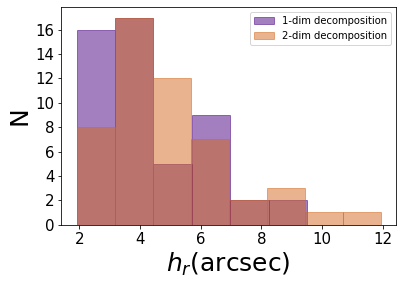
\includegraphics[width=.5\textwidth]{plot_results/h_arcsec.png}\hfill
    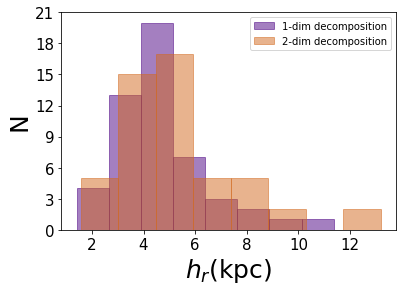
\includegraphics[width=.5\textwidth]{plot_results/h_kpc.png}\hfill\\
    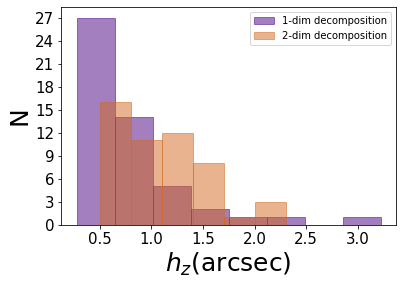
\includegraphics[width=.5\textwidth]{plot_results/h_z_arcsec.png}\hfill
    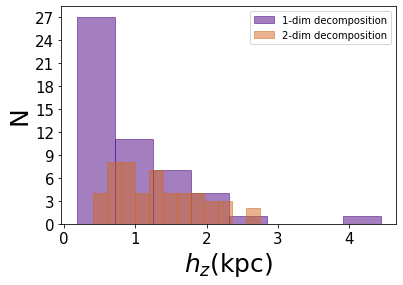
\includegraphics[width=.5\textwidth]{plot_results/h_z_kpc.png}\hfill\\

    \caption{Распределения по радиальным и вертикальным масштабам дисков галактик, выраженные в угловых секундах (левая панель) и в килопарсеках (правая панель). Цвет обозначает тип декомпозиции, в результате которой получены данные параметры: фиолетовый -- одномерная декомпозиция, оранжевый -- двумерная декомпозиция.}\label{fig:hz_hist}
\end{figure}

Получены средние значения радиальных масштабов диска: $\langle h \rangle_{1d}$ = $4.29 \pm 0.25$ arcsec и $\langle h \rangle_{2d}$ = $4.89 \pm 0.28$ arcsec, для одномерной и двумерной декомпозиции (в качестве ошибки здесь и далее приведено значение выборочной дисперсии).
Средние значения вертикальных масштабов диска $\langle h_z \rangle$ равны $0.79 \pm 0.08$ arcsec и $1.13 \pm 0.05$ arcsec также для одномерной и двумерной декомпозиции соответственно. Аналогично посчитаны
средние значения радиальных и вертикальных масштабов диска, выраженные в килопарсеках: $\langle h \rangle_{1d}$ = $4.72 \pm 0.27$ kpc и $\langle h \rangle_{2d}$ = $5.41 \pm 0.32$ kpc, для одномерной и двумерной декомпозиции. 
Средние значения вертикальных масштабов диска $\langle h_z \rangle$ равны $0.46 \pm 0.05$ kpc и $0.65 \pm 0.04$ kpc  для одномерной и двумерной декомпозиции соответственно. 
Приведенные значения масштабов выглядят типичными для наблюдаемых в ориентации с ребра близких галактик (см., например,
рис. 10 в \cite{2014ApJ...787...24B}).

Для получения значений масштабных параметров в килопарсеках из базы данных SDSS были взяты значения спектральных красных смещений для галактик выборки. При помощи красных смещений, используя пакет IMAN, мы смогли определить значения масштабов, связывающих размеры объектов, выраженные в угловых секундах с размерами, выраженными в килопарсеках. Распределение по красным смещениям для нашей выборки представлено на рис. \ref{fig:z_spec}. Все числовые величины в работе приведены для космологической
модели с постоянной Хаббла $H_0=70км\,c^{-1}\,\textrm{Мпк}^{-1}$, $\Omega_m=0.3, \Omega_{\Lambda}=0.7$.
\begin{figure}[th]
    \centering
    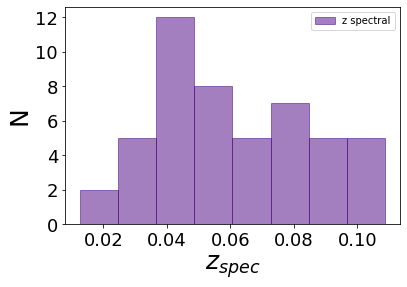
\includegraphics[width=.8\textwidth]{plot_results/z_spec.png}
    \caption{Распределение по спектральным красным смещениям галактик выборки, полученные из базы данных SDSS в фильтре r. }\label{fig:z_spec}
\end{figure}
Среднее красное смещение рассматриваемых нами галактик составляет $\langle z_{spec} \rangle$ = $0.064 \pm 0.004$. Галактики являются достаточно далекими для того, чтобы при дальнейших расчетах абсолютных звездных величин помимо галактического поглощения также учитывать значение К-поправки.

Распределение галактик по абсолютным звездным величинам (M) приведены на рис. \ref{fig:M_abs}.
\begin{figure}[th]
    \centering
    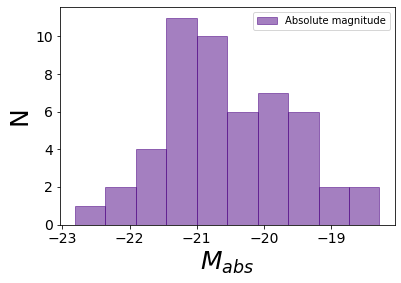
\includegraphics[width=.9\textwidth]{plot_results/M_abs.png}
    \caption{Распределение по абсолютным звездным величинам в фильтре r, расчитанным для модельных галактик. }\label{fig:M_abs}
\end{figure}
Абсолютные звездные величины были вычислены по формуле \ref{eq:M_abs}:
\begin{equation}
    M = m_{model}-5\log(D_L^{Mpc})-25-A-K,
    \label{eq:M_abs}
\end{equation}
Где $\textrm{ }m_{model}$ -- видимая звездная величина модельной галактики, $D_L^{Mpc}$(lumonocity distance) $=\sqrt{{\frac{L}{4\pi F}}}$ (где L -- светимость, F -- поток). Для расчета K-поправок использовался скрипт I. Chilingarian, A.-L. Melchior, and I. Zolotukhin. \footnote{http://kcor.sai.msu.ru/getthecode/}
Среднее значение M для галактик выборки: $\langle M \rangle_{2d}$ = $-20.53 \pm 0.13$, что согласуется с результатами работы \citep{2014ApJ...787...24B}.

% Изучаемая нами выборка видимых с ребра галактик в полосе Stripe 82 неполна. Эта неполнота должна сильнее всего проявляться для слабых и плохо разрешаемых галактик, у которых сложно определить ориентацию звездных дисков по отношению к лучу зрения.
О том, насколько галактика имеет тонкий звездный диск мы также можем судить по наблюдениям галактик, видимых с ребра. В большинстве своем, данная характеристика представляет собой отношения двух масштабных параметров \textit{h} и $z_0$ или \textit{h} и $h_z$. Существует четкая корелляция между этими двумя параметрами, что подтверждалось, например, в работах \citep{2002MNRAS.334..646K} или \citep{2010MNRAS.401..559M}. В нашей работе эта корреляция также присутствует (см. рис.\ref{fig:hr_z_0}). Примечательно, что продолжение линейной регрессии проходит вблизи точки с координатами (0, 0). 

Мы также построили распределение толщин звездных дисков для одномерной и двумерной декомпозиции \ref{fig:hr_hz_hist}. Видим, что существует большой разброс значений $h/z_0$ по результатам одномерной декомпозиции, в то время, как $h/z_0$ для двумерной декомпозиции ограничивается значением$\approx$ 9.5. Считаем, что данная несостыковка произошла из-за неточного определения значения $z_0$ в процессе одномерной декомпозиции, как минимум значения толщин $h/z_0 \approx$ 20.0 -- нефизичны. Еще одно подтверждение того, что одномерную декомпозицию лучше использовать исключительно в качестве начального приближения для двумерной.  
\begin{figure}[th]
    \centering
    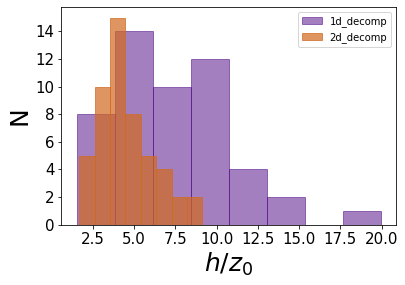
\includegraphics[width=.8\textwidth]{plot_results/h_z0_hist.png}
    \caption{Распределение галактик по значениям толщин звездных дисков. Фиолетовая гистограма демонстрирует параметры, полученные в процессе одномерной декомпозиции, оранжевая гистограмма -- в процессе двумерной. }\label{fig:hr_hz_hist}
\end{figure}

\begin{figure}[th]
    \centering
    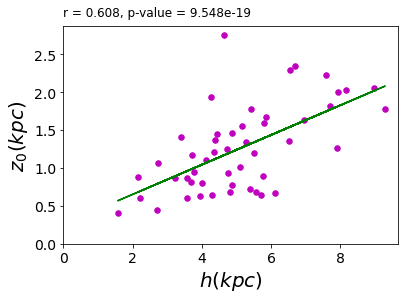
\includegraphics[width=.8\textwidth]{plot_results/h_r_z_0.png}
    \caption{Распределение галактик на плоскости $h$ $h_z$, зеленая сплошная линия -- линейная регрессия для данной выборки галактик, r -- коэффициент Пирсона, p -- p-значение. }\label{fig:hr_z_0}
\end{figure}

Заключительный и наиболее важный раздел анализа, выполненный в рамках данной работы, это анализ толщин звездных дисков галактик в зависимости от наличия или отсутствия у тех приливных структур. Из теоретических соображений следует, что толщина звездных дисков чувствительна к внешнему возмущению и аккреции вещества \cite{1992ApJ...389....5T}. При гравитационном взаимодействии галактик, в частности, при малых и больших слияниях, часть энергии орбитального движения галактик может преобразоваться в их внутреннюю энергию, "разогреть"$\textrm{ }$ звездные диски, тем самым увеличив дисперсию скоростей звезд в вертикальном направлении, следовательно, и наблюдаемую толщину. Эффект приливного утолщения был, действительно, открыт при сравнении распределений яркости в вертикальном направлении в выборках взаимодействующих и относительно изолированных галактик в работе \citep{1997A&A...324...80R}. Было продемонстрировано, что галактики во взаимодействующих системах демонстрируют в 1.5-2 раза более толстые диски по сравнению с галактиками в более бедном пространственном окружении. Мы решили проверить этот факт на нашей выборке. В данном случае речь идет о всем каталоге галактик EG82, содержащем 831 объект, так мы имеем возможность учесть все галактики из предыдущего раздела, посвященного приливным структурам. В качестве критерия оценки толщин дисков мы будем использовать отношение полуосей \textit{b/a}. Соответственно, чем меньше это соотношение, тем тоньше диск, и на оборот. На 831 объект выборки у нас приходится 43 галактики с наблюдаемыми приливными структурами. Мы построили распределение толщин для двух подвыборок: галактик с приливными структурами и оставшейся части выборки (788 объектов) (см. рис. \ref{fig:b_a}.) 
\begin{figure}[th]
    \centering
    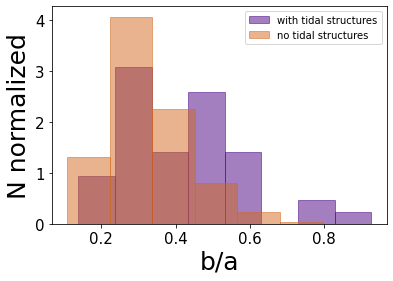
\includegraphics[width=.8\textwidth]{plot_results/b_a.png}
    \caption{Распределение толщин галактик (отношение малой полуоси к большой) для двух выборок галактик: фиолетовая гистограмма для галактик с наблюдаемыми приливными структурами, оранжевая гистограмма для галактик с отсутствующими приливными структурами.}\label{fig:b_a} 
\end{figure}

Среднее значение толщины диска для выборки с приливными структурами -- $\langle b/a \rangle_{2d}$ = $0.412 \pm 0.03$, в то время, как для выборки галактик, у которых приливные структуры отсутствуют это же значение равно  $\langle b/a \rangle_{2d}$ = $0.325 \pm 0.003$. Не в два раза, но все равно диски галактик со структурами заметно толще дисков визуально не взаимодействующих галактик.
    % \item Исходя из графика, представленного на рисунке (??) мы можем сделать вывод о наличие корелляции между параметрами $h_r$ и $z_0$. Отметим тот факт,что график линейной функции, аппроксимирующий распределение в пространстве данных параметров проходит через точку, близкую к точке с координатами (0,0).  Среднее значение отношения $h_r/z_0$ для одномерной и двумерной декомпозиции: $\langle h_r/z_0 \rangle_{1d}=$  $7.40 \pm 0.43$ и $\langle h_r/z_0 \rangle_{1d} =$  $4.97 \pm 0.23$.
    % \item 

\section{Заключение}
\begin{itemize}
    \item В рамках данной работы был создан каталог галактик с ребра в SDSS полосе Stripe 82 -- \textit{SG82.} Каталог на данный момент содержит 831 объект, включая галактики с углом наклона меньше 85\degree (визуально), 710 объектов, если исключить галактики, не являющиеся галактиками с ребра.
    \item Был проведен тест $V/V_m$ на полноту выборки. Для галактик с размером большой полуоси $SMA>18$ arcsec наша выборка, по существу, полна: в фильтре \textit{r} $\langle V/V_m \rangle = 0.489$.
    \item Были уточнены такие параметры галактик из каталога, как размеры полуосей и позиционные углы.
    \item Обработаны изображения объектов из каталога в фильтрах g, r, i, rdeep. 
    \item Получены цветные RGB и суммарные изображения.
    \item Отобрано и проклассифицировано 43 галактики, обладающие приливными LSB структурами, 86 галактик обладает структурными особенностями, не являющимися приливными. Важный результат этой работы заключается в том, что несмотря на глубину исследуемых изображений, количество галактик, обладающих структурами низкой поверхностной яркости в выборке намного меньше, чем ожидалось. Возможно глубины исследуемых данных недостаточно, чтобы выявить все галактики с приливными структурами и структурными особенностями.
    \item Выполнена одномерная фотометрическая декомпозиция для 73 галактик, для 51 галактики результаты фотометрической декомпозиции оказались хорошими или удовлетворительными. Оставшиеся 22 галактики либо не являются галактиками, видимыми точно с ребра, либо нуждаются в более сложных моделях для аппроксимации (например 3D модели с изломами диска). 
    \item Был произведен анализ масштабных параметров и сделаны оценки их средних значений. Средние значения вертикального и радиального масштабов, а также средние абсолютные звездные величины согласуются с результатами ранее выполненных работ других авторов. На основании графиков еще раз был подтвержден факт о наличии корреляции между радиальным и вертикальным масштабами диска, 
    \item Для всех галактик с результатами анализа распределения яркости выполнены отождествления с опубликованными списками спектральных красных смещений. Среднее красное смещение галактик выборки оказалось равным $\approx$ 0.064.
    \item Показано, что звездные диски галактик с наблюдаемыми приливными структурами в среднем являются более толстыми, чем диски галактик, у которых эти структуры отсутствуют.

\end{itemize}

Составленный каталог галактик можно в дальнейшем использовать для более подробного анализа структур низкой поверхностной яркости. Полученные результаты находятся в согласии с современными представлениями об эволюции дисковых подсистем галактик. Результаты дипломной работы дают важную информацию о структуре взаимодействующих галактик и они могут быть использованы для дальнейшего исследования фотометрических параметров и эволюции подсистем. 

\section*{Благодарность}

В заключение, я хочу выразить благодарность своему научному руководителю за постановку актуальной и интересной задачи, сопровождение на всем пути написания дипломной работы, конструктивную обратную связь, за понимание и помощь в освоении нового теоретического материала и программ. Благодарю сотрудников кафедры астрофизики за ценные замечания и обсуждение вопросов, связанных с дипломной работой и обучением в целом. Также хочу поблагодарить всех преподавателей университета за переданные знания и опыт, которые помогли мне получить качественное образование и привить любовь астрономии, математике и другим точным наукам. И я очень благодарна своей семье и университетским друзьям, которые поддерживали меня на протяжении всего периода обучения в университете. 
\newpage
\bibliographystyle{abbrv}
\bibliography{reference}



\end{document}